\documentclass[twocolumn, linenumbers]{aastex631}
\usepackage{graphicx}
\usepackage{physics}
\usepackage[super]{nth}
\usepackage{enumitem}
\usepackage[all]{hypcap}

\makeatletter
\renewcommand\hyper@natlinkbreak[2]{#1}
\makeatother

\begin{document}
\title{A New Hybrid Machine Learning Method for Stellar Parameter Inference}
\author[0000-0002-2290-6810]{Sujay Shankar}
\correspondingauthor{Sujay Shankar}
\email{sujays2001@gmail.com}
\author[0000-0002-4020-3457]{Michael A. Gully-Santiago}
\author[0000-0002-4404-0456]{Caroline V. Morley}
\affil{Department of Astronomy, The University of Texas at Austin, Austin, TX 78712, USA}

\shorttitle{HML for Stellar Parameter Inference}

\begin{abstract}
    The advent of machine learning (ML) is revolutionary to numerous scientific disciplines, with a growing number of examples in astronomical spectroscopic inference, as ML is expected to be more powerful than traditional techniques.
    Here we introduce a hybrid ML (HML) method combin{ing} automatic differentiation, interpolation, and Bayesian optimization to infer stellar parameters given stellar spectra.
    We study $T_{\mathrm{eff}}$, $\log(g)$, and [Fe/H], but this method \textbf{could be extended} to other \textbf{parameters} such as [$\alpha$/Fe] \textbf{(alpha element abundance)}, C/O \textbf{(carbon-oxygen ratio)}, and $f_{sed}$ \textbf{(sedimentation efficiency)}.
    We first use \texttt{blase}'s nontraditional semi-empirical approach, \textbf{recasting} spectra \textbf{into} sets of tunable spectral lines.
    \texttt{blase} is \textbf{run} on 1,314 spectra from \textbf{a rectilinear subset of} the PHOENIX synthetic spectral model grid \textbf{([Fe/H]: [-0.5, 0] dex, $T_\text{eff}$: [2300, 12000] K, $\log(g)$: [2, 6])}.
    For each of the \textbf{128,723} lines, we continuously map stellar parameters to spectral line parameters using regular grid linear interpolation.
    These manifolds are aggregated to create the PHOENIX generator, \textbf{enabling} parallelized reconstruction of spectra given stellar parameters.
    Gaussian Process minimization is then used to infer stellar parameters by minimizing the root-mean-square (RMS) loss between input and PHOENIX generator spectra.
    From testing, the inference error in $T_{\mathrm{eff}}$ was 185 K, $\log(g)$ was 0.19, and [Fe/H] was 0.12 dex.
    Our products are an archive of the \texttt{blase} \textbf{models} of the PHOENIX subset, as well as the spectral reconstruction and inference algorithms themselves.
    This study is a proof of concept showing that semi-empirical HML is a viable alternative to traditional approaches.
\end{abstract}

\section{Introduction}
Stellar spectra are exceedingly rich sources of information about the stars that produce them.
Spectra encode fundamental properties such as temperature, surface gravity, and chemical composition via their numerous absorption lines.
Extrinsic properties such as the stellar radial velocity or the projected equatorial rotation shift the wavelengths of lines and broaden their widths, respectively.
Observing the spectrum alters it again; the resolution, bandwidth, and other properties of the instrument change the fidelity at which we observe the spectrum, and can limit our ability to extract fundamental properties precisely.
Observed stellar spectra thus represent extremely complex, data, influenced by multiple parameters, that have gone through multiple transformations before reaching our detectors.

Modern astronomical spectroscopy \textbf{takes advantage of intuitive, performant spectral models such as KORG \citep{korg}, however it} would \textbf{further} benefit from \textbf{the paradigm of interpretability}.
The determination of fundamental properties, the creation of Extreme Precision Radial Velocity (EPRV) templates, and the application of composite spectral fitting could all leverage such an innovation.
This ambitious aim may be broadly referred to as a ``foundational spectroscopy model for astrophysics'', in reference to the same category of models used for large language models (LLMs) in artificial intelligence (AI).
There are many challenges with creating such a foundational spectral model for astrophysics.
Physical inputs into the spectral modeling process are imperfect\textbf{, and} simplifying assumptions in stellar (and substellar) atmospheres are necessarily inexact \textbf{due to factors such as asymmetries and unknown physics}.
Computational costs \textbf{make} the training of such models \textbf{challenging; however, advances have been made with attention-based \citep{foundation_attention} and transformer-based \citep{foundation_transformer} models, among others}.
Most prevailing solutions have had to choose either a model driven approach \textbf{(such as this work)}, in which precomputed models are taken as gospel, or a data driven/empirical approach \textbf{(such as Lux \citep{lux})}, in which our knowledge of stellar physics is ignored or treated phenomenologically, depending on the application.
\textbf{Hybrid solutions exist and have been implemented, such as those presented in \citealt{leung2019} and \citealt{rains2024}.
Although a lingering challenge is always how to ideally balance the fusion of model driven and data driven paradigms.}

Spectroscopic surveys such as APOGEE \textbf{\citep{APOGEE}} use their own in-house pipelines to extract stellar parameters from spectra (ASPCAP \textbf{\citep{ASPCAP}} in the case of APOGEE), and these pipelines appear effective.
The core assumption for the vast majority of pipelines is that the data to be analyzed is a list of pixels.
Analysis pipelines may be closed-source or limited to the scope of the survey itself, causing a sort of siloing effect among surveys.
This motivates the development of more universal, instrument-agnostic open-source frameworks that can apply broadly to a range of spectral observations with relatively little tuning.

Multiple efforts have been made in this direction, treating spectra in different ways.
The standard practice is to treat the wavelength and flux as simply two arrays and use bespoke algorithms tailored to a small number of well-calibrated spectral lines to obtain fundamental stellar parameters and chemical compositions \citep{pipeline1, pipeline2}.
Other whole-spectrum fitting abstractions decompose model spectra into an eigenbasis, implementing the data-model comparison stage as a tractable regression, such as \texttt{starfish} \citep{starfish}.

Ideally, we want a system that can self-consistently learn, a genuine AI foundational spectral model.
Such a system would enable the assignment of accurate stellar parameters, and could yield re-usable interpretable spectral models.
\texttt{blase}, first presented in \citealt{blase}, took an important, albeit limited, step in this direction, treating spectra not as a set of pixels or a set of eigenbasis coefficients but as a set of interpretable and traceable spectral lines, specifically Voigt profiles.
Each of these approaches has tradeoffs, but one key scientific advantage of \texttt{blase} comes from its ability to adapt to new information, while preserving some adherence to physics-based models.
This intelligent capability stems from its ability to fit a theoretically unlimited number of nonlinear spectral line parameters with automatic differentiation (autodiff).
Autodiff is a technology that tracks transformations made to data using the chain rule, even being able to differentiate control flow transformations involving if-else blocks, for example.
With the gradient obtained from autodiff's chain rule, we can optimize model parameters by just going against the direction of the gradient (because we usually want to minimize something such as a loss function, we go in the direction of greatest decrease, which is always the negative of the gradient).
Autodiff has been used successfully in other astrophysical contexts such as \texttt{exojax} \textbf{\citep{exojax}} and \texttt{wobble} \citep{wobble}, but the recasting of spectra into sets of inherently nonlinear spectral lines positions \texttt{blase} as a unique and promising semi-empirical tool.
The original \texttt{blase} paper demonstrated the ability to tune spectral lines with autodiff \textbf{and `clone' spectra, recasting them as ML models defined by interpretable sets of tuned spectral lines, however it was} restricted to a pre-selected static synthetic model.

Here we introduce the next logical step in the sequence of expanding interpretable spectroscopic machine learning from operating on a single grid point and towards an entire 3D grid of precomputed spectra.
We rebrand this augmentation as \texttt{blase3D}.

Ideally this process would be monolithic, with the end-to-end spectral inference code powered by a single autodiffable machine learning framework, like PyTorch \textbf{\citep{pytorch}} or JAX \citep{jax}.
However, here we separate the problem into three pieces, only the first of which is currently differentiable.
\textbf{In \autoref{sec:section2},} we scale out the \texttt{blase} method to 1,314 precomputed synthetic spectral model clones, yielding a downloadable archive of pretrained machine learning models with 128,723 unique spectral lines.
\textbf{In \autoref{sec:section3},} we \textbf{then} fit manifolds mapping stellar parameters to uniformly-derived spectral line parameters using regular grid linear interpolation.
Finally, \textbf{in \autoref{sec:section4},} we show how reconstructions of the spectra using said manifolds can be used for inferring stellar fundamental properties from spectra.
This final step resembles the aims of ``atmospheric retrievals'', but in principle should be faster, adaptive, and reusable.
An overview of this process is shown in \autoref{fig:figure1}.

\begin{figure*}
    \centering
    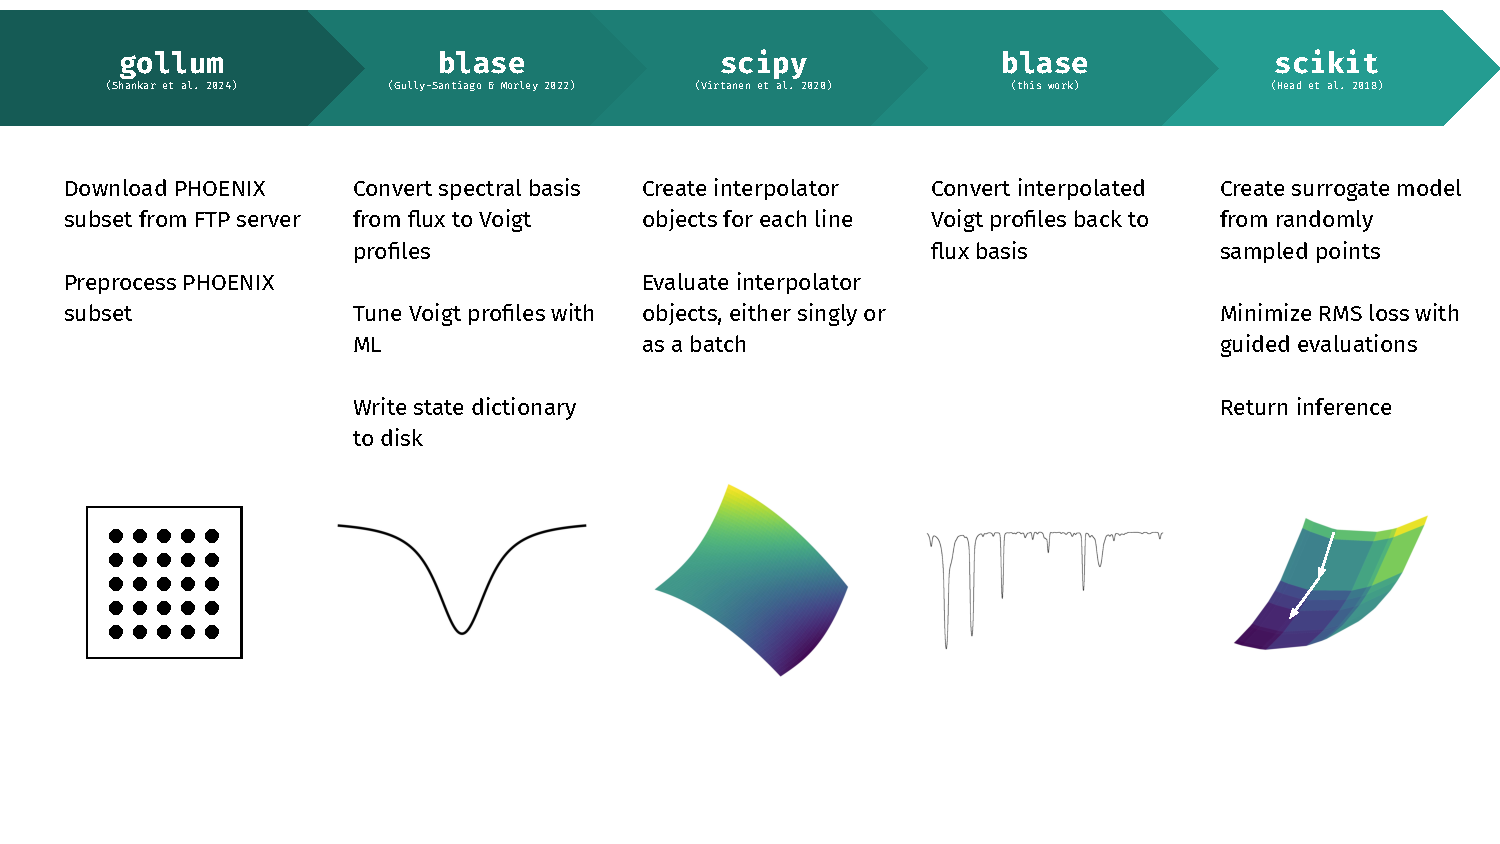
\includegraphics[width=\textwidth]{figure1}
    \caption{Overview of the process used in this study.}
    \label{fig:figure1}
\end{figure*}


\section{Cloning the PHOENIX Model Grid}
\label{sec:section2}
\subsection{The PHOENIX Subset}
\textbf{For the purposes of this study, w}e chose the widely-adopted PHOENIX synthetic spectral model grid \citep{PHOENIX}.
Our approach can be straightforwardly applied to any other model grid in the future, including substellar atmosphere grids such as Sonora \citep{bobcat, cholla, diamondback, elfowl}, but for now we limit our scope to a \textbf{rectilinear} subset of the PHOENIX grid, focusing on near solar metallicities and a broad range of effective temperature and surface gravity, with details given in \autoref{tab:table1}.
\textbf{This approach is taken due to the computational cost of interpolation algorithms.
Future versions with more advanced models will be able to bypass the limitation of a rectilinear subset.}

\begin{table*}
    \hspace*{0.6cm}\begin{tabular}{llll}
        \hline
        \bf{Parameter} & \bf{Symbol} & \bf{Interval} & \bf{Sampling}\\
        \hline
        Alpha Element Abundance & $\alpha$ & [0] dex & \bf{N/A}\\
        Iron Abundance & [Fe/H] & [-0.5, 0] dex & \bf{0.5 dex}\\
        Effective Temperature & $T_{\mathrm{eff}}$ & [2300, 12000] K & \bf{100 K until 7000 K, then 200 K}\\
        Surface Gravity & $\log(g)$ & [2, 6] & \bf{0.5} \\
        Wavelength & $\lambda$ & [8038, 12849] \AA & $\mathbf{R = 500,000}$\\
        \hline
    \end{tabular}
    \caption{The subset of the PHOENIX grid used in this study.
    These limits were imposed to reduce the computational cost of the algorithms and to ensure a rectilinear parameter space in order to work with \texttt{scipy}'s \texttt{RegularGridInterpolator} \citep{scipy}.
    The wavelength limits in particular roughly line up with that of the Habitable Zone Planet Finder (HPF) spectrograph \citep{HPF}.
    This subset is comprised of 1,314 individual spectra: 73 $T_{\mathrm{eff}}$ values, 9 $\log(g)$ values, and 2 [Fe/H] values.}
    \label{tab:table1}
\end{table*}

\subsection{Preprocessing with \texttt{gollum}}
First, the PHOENIX subset was programmatically retrieved with \texttt{gollum} \textbf{\citep{gollum}}, which downloaded \textbf{spectra} from the PHOENIX FTP server. The spectra were then put through a
three-step preprocessing pipeline similar to that from \citealt{blase}.
\begin{enumerate}
    \item \textit{Blackbody Division}: Since the $T_{\mathrm{eff}}$ of each spectrum is known, the \textbf{corresponding} blackbody spectrum was divided out.
    \item \textit{Percentile Normalization}: The spectra were normalized by dividing them by their 99th percentile in order to collapse the dynamic range of flux and only look at relative features.
    \item \textit{Continuum Normalization}: The spectra were further normalized by dividing them by a \nth{5} order polynomial continuum fit using a peak-finding filter in order to eliminate curvature that would inhibit line modeling.
\end{enumerate}
Mathematically, we can express the preprocessing as follows:
\begin{linenomath*}
\begin{gather}
    \mathsf{\bar{S}} = \dfrac{\mathsf{S}}{\mathsf{B}\mathsf{Q}_5P_{99}}
\end{gather}
\end{linenomath*}
where $\mathsf{\bar{S}}$ is the preprocessed spectrum, $\mathsf{S}$ is the original spectrum,  $\mathsf{B}$ is the blackbody spectrum, $\mathsf{Q}_n$ is the $n^\mathrm{th}$ order polynomial continuum fit, and $P_n$ is the $n^\mathrm{th}$ percentile function.
Arithmetic operations between arrays are assumed to be elementwise in all following notation.

\subsection{Line Identification with \texttt{blase}}
The next step was to convert the PHOENIX subset into a physically interpretable intermediate representation: a table of spectral line properties rather than a\textbf{n} array of fluxes.
We used \texttt{blase}, which models spectral lines as Voigt profiles and tunes the profiles to mimic the original PHOENIX spectrum with back propagation.
Back propagation, put simply, is the process of moving in the autodiff gradient field to update ML model parameters (like mentioned earlier, usually against the gradient because we minimize loss functions).
Four parameters were optimized: the line center $\mu$, the log-amplitude $\ln(a)$, the Gaussian width $\sigma$, and the Lorentzian width $\gamma$.
The optimization used the Adam optimizer \textbf{\citep{adam}} with a learning rate of 0.05 over 100 epochs.
\textbf{\citealt{blase} recommends this setup as the minimum, and for a proof-of-concept implementation, we found it best to leave it as is.}
In addition, we limited two custom parameters: wing cut to 6000 and prominence to 0.005.
Wing cut \textbf{(in pixels)} is a parameter that determines the extent of the Voigt profile to evaluate, saving computational resources by not evaluating negligible line wings.
Prominence \textbf{(in normalized flux counts)} sets a lower limit for the amplitude of detected lines, which saves resources by disregarding shallow lines, so in our case we disregard lines \textbf{with amplitude} $<$ 0.05.
In short, our choices for wing cut and prominence decrease the computational cost of \texttt{blase}'s cloning process at the expense of decreasing its accuracy slightly.
\texttt{blase} uses the pseudo-Voigt approximation, which saves on computational cost while remaining accurate to about 1\% \citep{pseudovoigt}.
The pseudo-Voigt approximation uses a weighted average of a Gaussian and Lorentzian as opposed to a convolution.
\texttt{blase}'s pseudo-Voigt profile implementation uses the following:
\begin{linenomath*}
\begin{subequations}
\begin{gather}
    \tilde{\mathsf{V}}_\mu(\lambda) = a\left[\eta \mathbf{L}(\lambda - \mu'; f) + (1 - \eta)\mathbf{G}(\lambda - \mu'; f)\right]\\
    \eta = \sum_{n=1}^3 \mathbf{u}_n\left(\dfrac{2\gamma}{f}\right)^n\\
    f = 32\sum_{n=0}^5 \mathbf{v}_n \left(\sqrt{2\ln(2)}\sigma\right)^{5-n}(\gamma)^n\\
    \nonumber \mathbf{u} = \mqty[1.36603 \\ -0.47719 \\ 0.11116] \quad \mathbf{v} = \mqty[1 \\ 2.69269 \\ 2.42843 \\ 4.47163 \\ 0.07842 \\ 1]
    \label{eq:equation2}
\end{gather}
\end{subequations}
\end{linenomath*}
where $\mathbf{L}$ and $\mathbf{G}$ are abbreviations for Lorentzian and Gaussian profiles, respectively.
Notice that we use $\mu'$ instead of $\mu$ in the formula.
This is because \texttt{blase} optionally allows the line center to shift slightly during optimization, and it is this shifted center which is used in computation.
The individual Voigt profiles are still indexed by $\mu$ for cross-model line identification, explained in the next section.
Once optimization was complete, the list of identified lines was saved to a `state dictionary': a common representation for pre-trained machine learning models that can be stored to disk for reuse later.
These are stored in the \texttt{.pt} file format for each of the 1,314 PHOENIX subset grid points.
The total disk space these files take up is 465 MB (382 MB when downloaded as a zip archive).
For reference, the storage space the PHOENIX subset takes up on disk is approximately 8.1 GB.
This represents a data compression factor of around 20 just by recasting the spectrum with \texttt{blase}.
\textbf{The state dictionaries are available on Zenodo at \url{https://zenodo.org/records/11246174} \citep{zenodo}.}

\section{Interpolating Manifolds}
\label{sec:section3}
\subsection{Cross-Model Line Identification}
As previously mentioned, \texttt{blase} tunes the line centers of detected lines.
This means that from one PHOENIX spectrum to the next, the same line could have a slightly different line center.
Since the goal of this study is to interpolate the properties of each line, we needed to identify the presence of a particular line across the PHOENIX subset, associating the same line with every occurrence.
We decided to do this by using the line centers $\mu$ of the detected lines pre-optimization.
Now with each spectral line indexed by $\mu$, we had four parameters to interpolate: $\mu'$, $\ln(a)$, $\sigma$, and $\gamma$.
Note that since we are dealing with the parameters of Voigt profiles, we can see in \autoref{eq:equation2} that even if the interpolation method is linear, a final spectral reconstruction will vary nonlinearly in flux.

Spectral lines were often only detected in some spectra from the PHOENIX subset.
In \autoref{fig:figure2}, we show that different grid points \textbf{show} differing counts of detected spectral lines.
\begin{figure*}
    \centering
    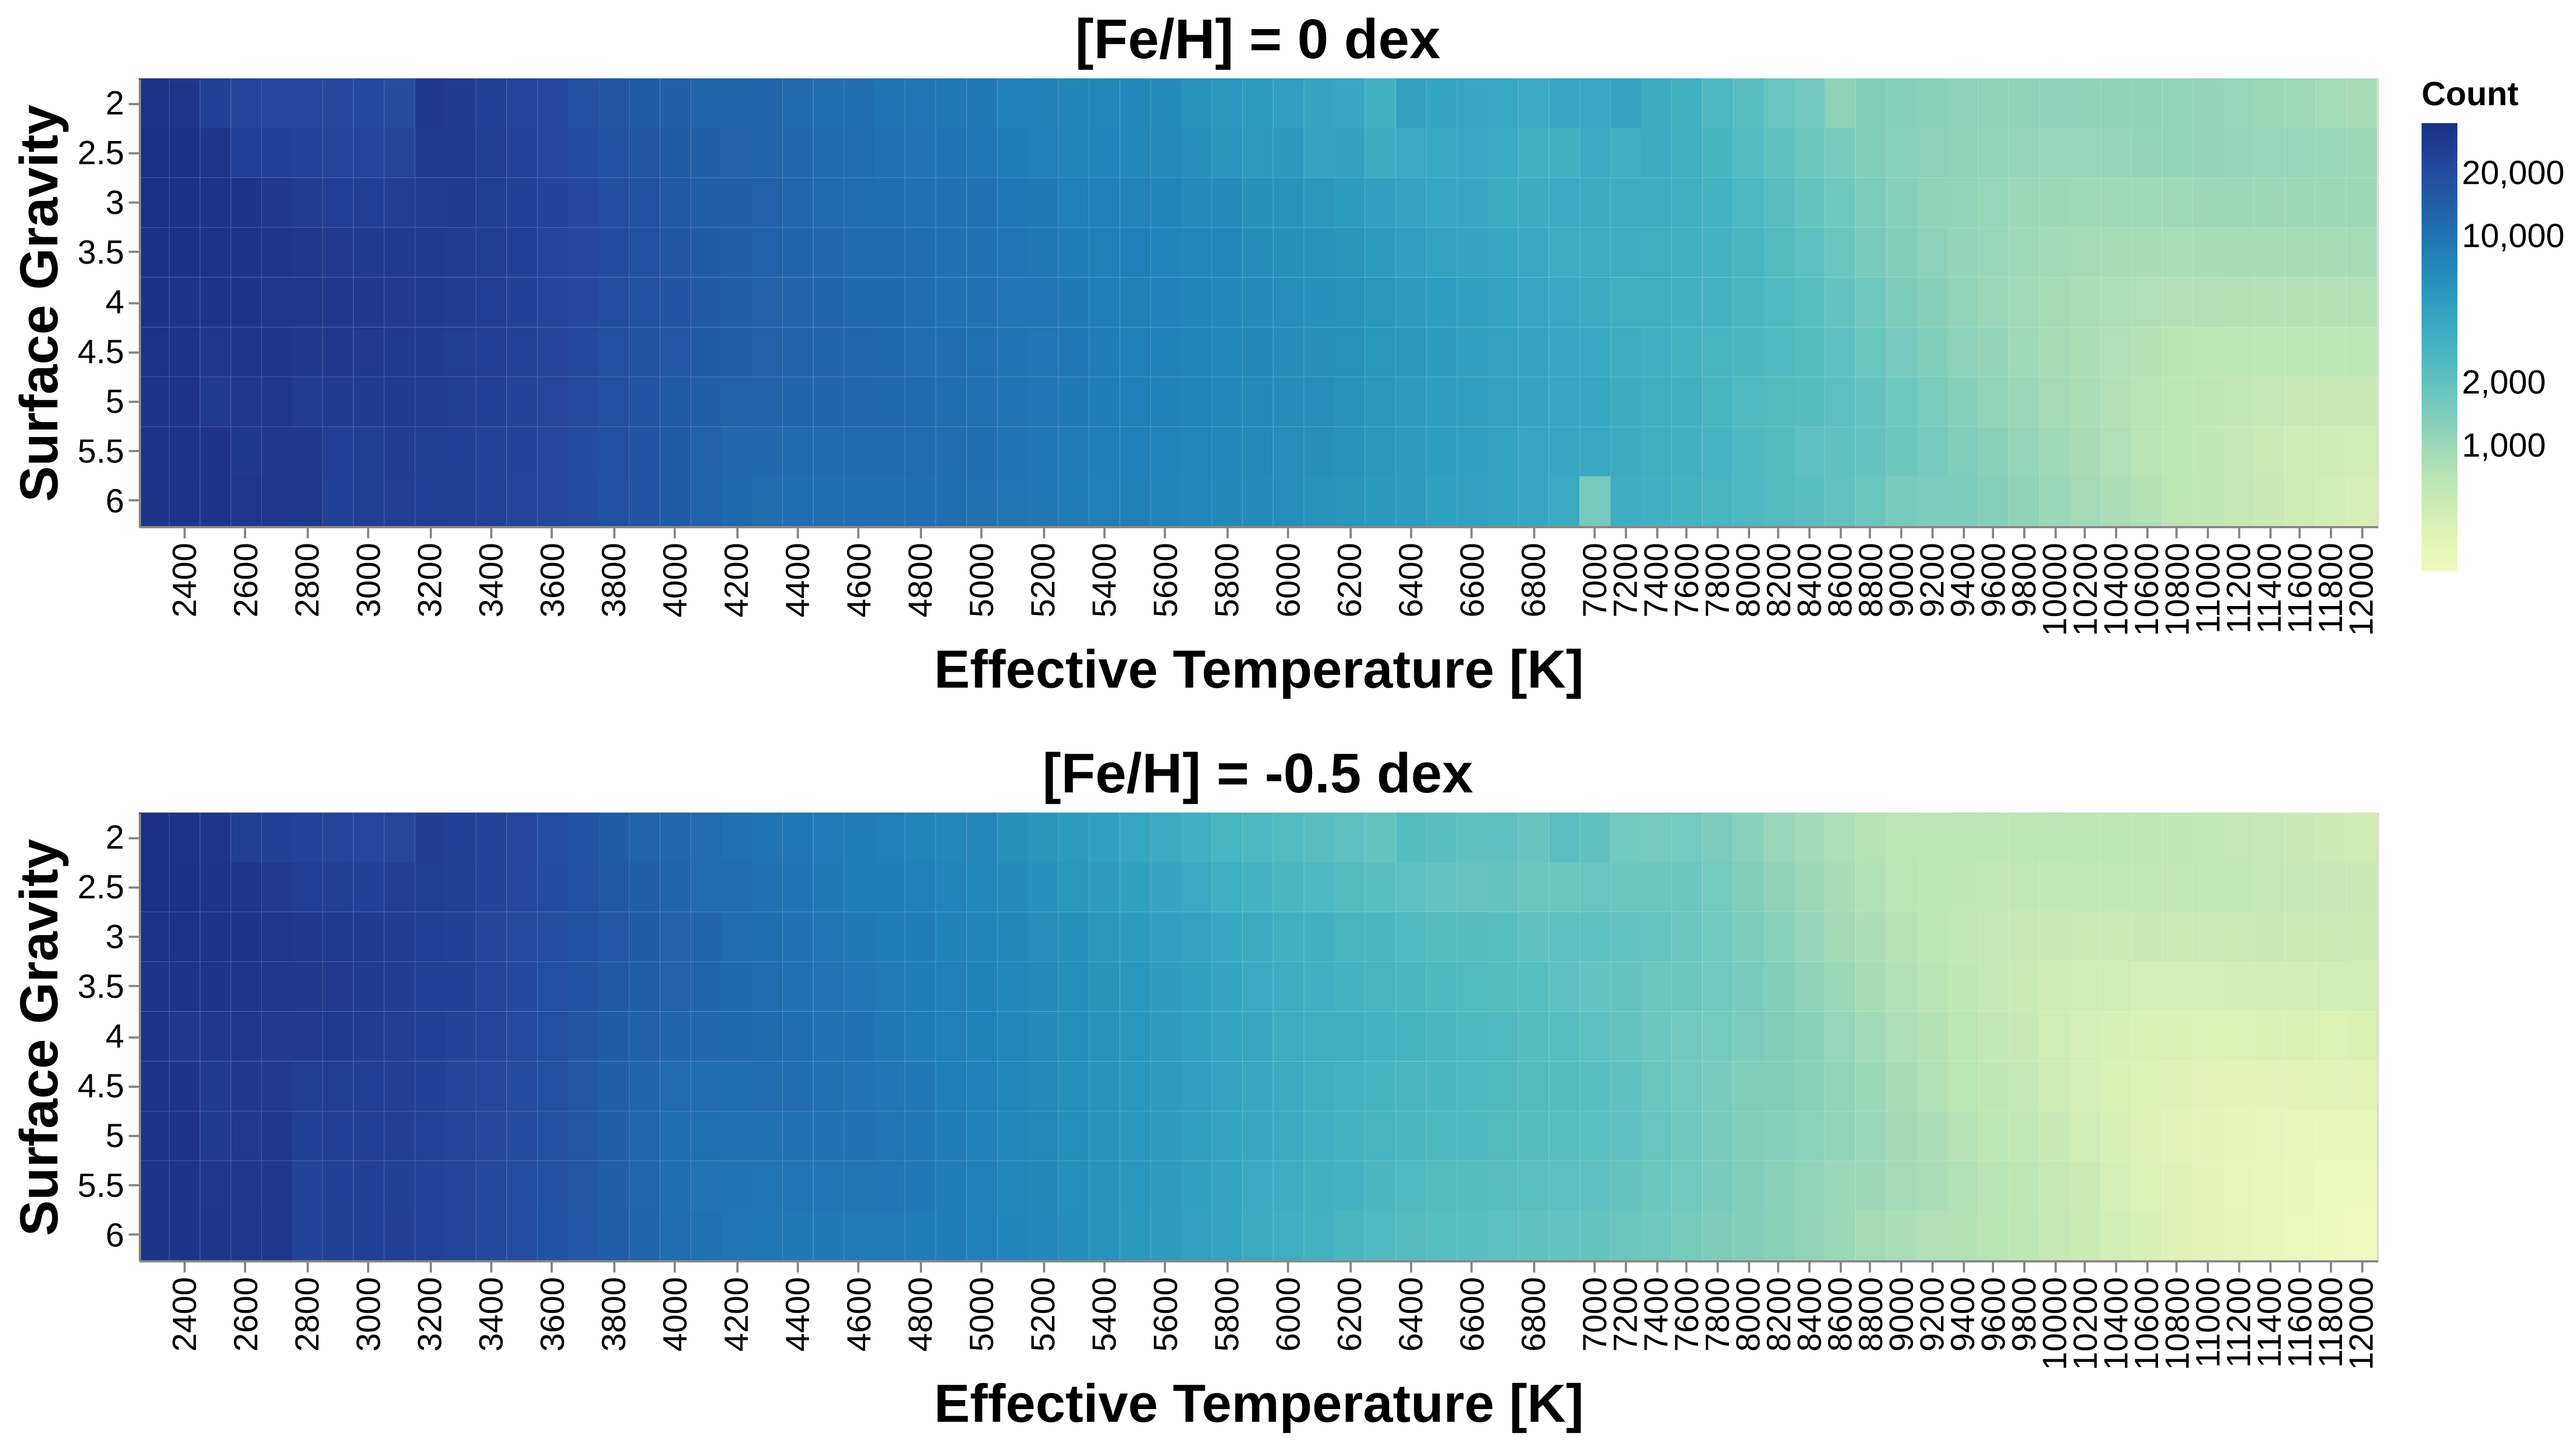
\includegraphics[width=\textwidth]{figure2}
    \caption{Number of detected spectral lines at each grid point of a slice of the PHOENIX subset at solar metallicity.
    We can see that the number of detected lines decreases with increasing $T_{\mathrm{eff}}$.
    Also note that from $T_{\mathrm{eff}} = 7000$ K onward, PHOENIX's sampling increment changes from 100 K to 200 K.}
    \label{fig:figure2}
\end{figure*}

Th\textbf{e number of detected spectral lines changes as a function of stellar parameter} for different reasons.
Perhaps for astrophysical reasons: stellar atmospheres genuinely do not produce that line at detectable strength at the given temperature and surface gravity.
Or alternatively, our line-finding and line-association algorithms missed it.
Whatever the cause, these missing lines have immediate practical consequences.
Rectilinear interpolation schemes break in regions where a line does not appear; you can't interpolate a quantity that simply doesn't exist.

To solve this, we artificially populated missing grid points with log-amplitudes of -1000, which retained interpolator stability while nullifying the evaluated line.
Examples of the appearance of missing sections in heatmaps where a line does not appear are shown in \autoref{fig:figure3} and \autoref{fig:figure4}.
In total, across the entire PHOENIX subset, \texttt{blase} detected 128,723 individual spectral lines.
Every one of these lines can be visualized as a manifold mapping a 3D stellar parameter vector to a 4D spectral line parameter vector, and every one \textbf{was} interpolated \textbf{to map stellar parameters to spectral line properties}.
\begin{figure*}
    \centering
    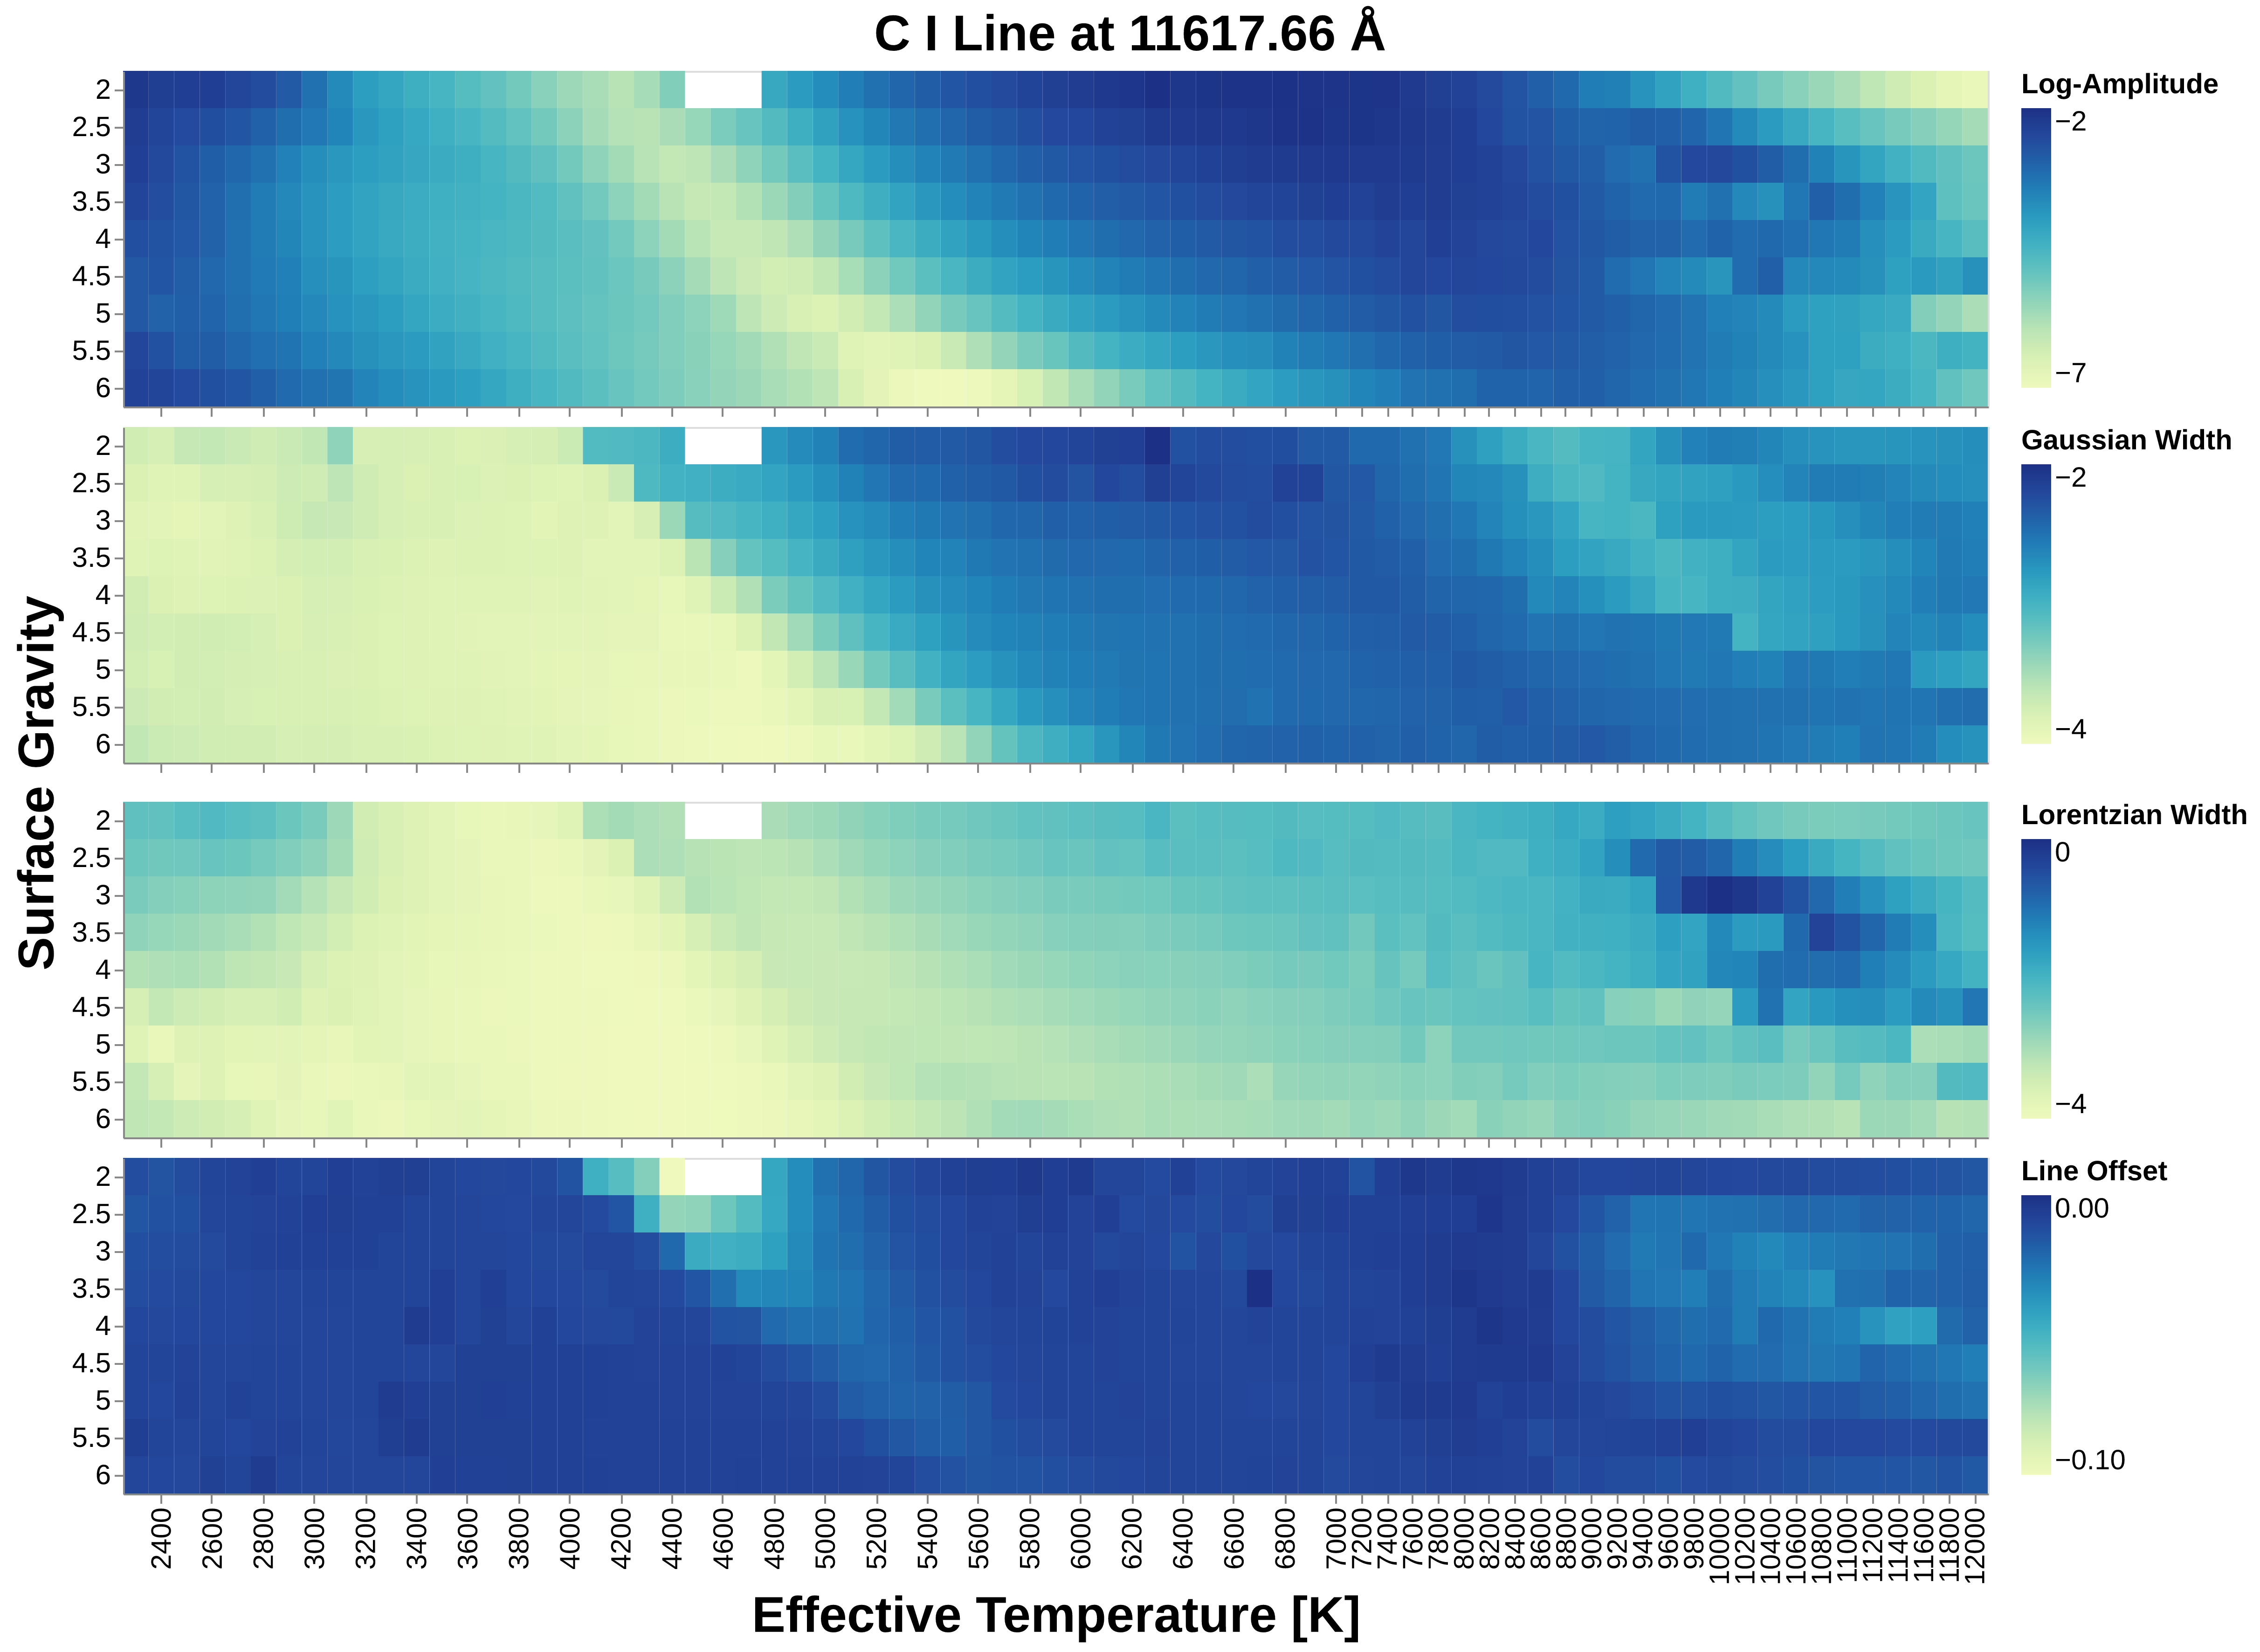
\includegraphics[width=\textwidth]{figure3}
    \caption{Heatmap showing how $\ln(a)$ and $\sigma$ vary over the PHOENIX subset slice at solar metallicity of a \textbf{C I} spectral line.
    Notice the missing chunk in the top left of the figure; \texttt{blase} did not detect a spectral line here, but we have to artificially populate those points with lines that have $\ln(a) = -1000$.
    This and all spectral lines shown in this paper were identified using the NIST spectral line database \citep{NIST}.}
    \label{fig:figure3}
\end{figure*}
\begin{figure*}
    \centering
    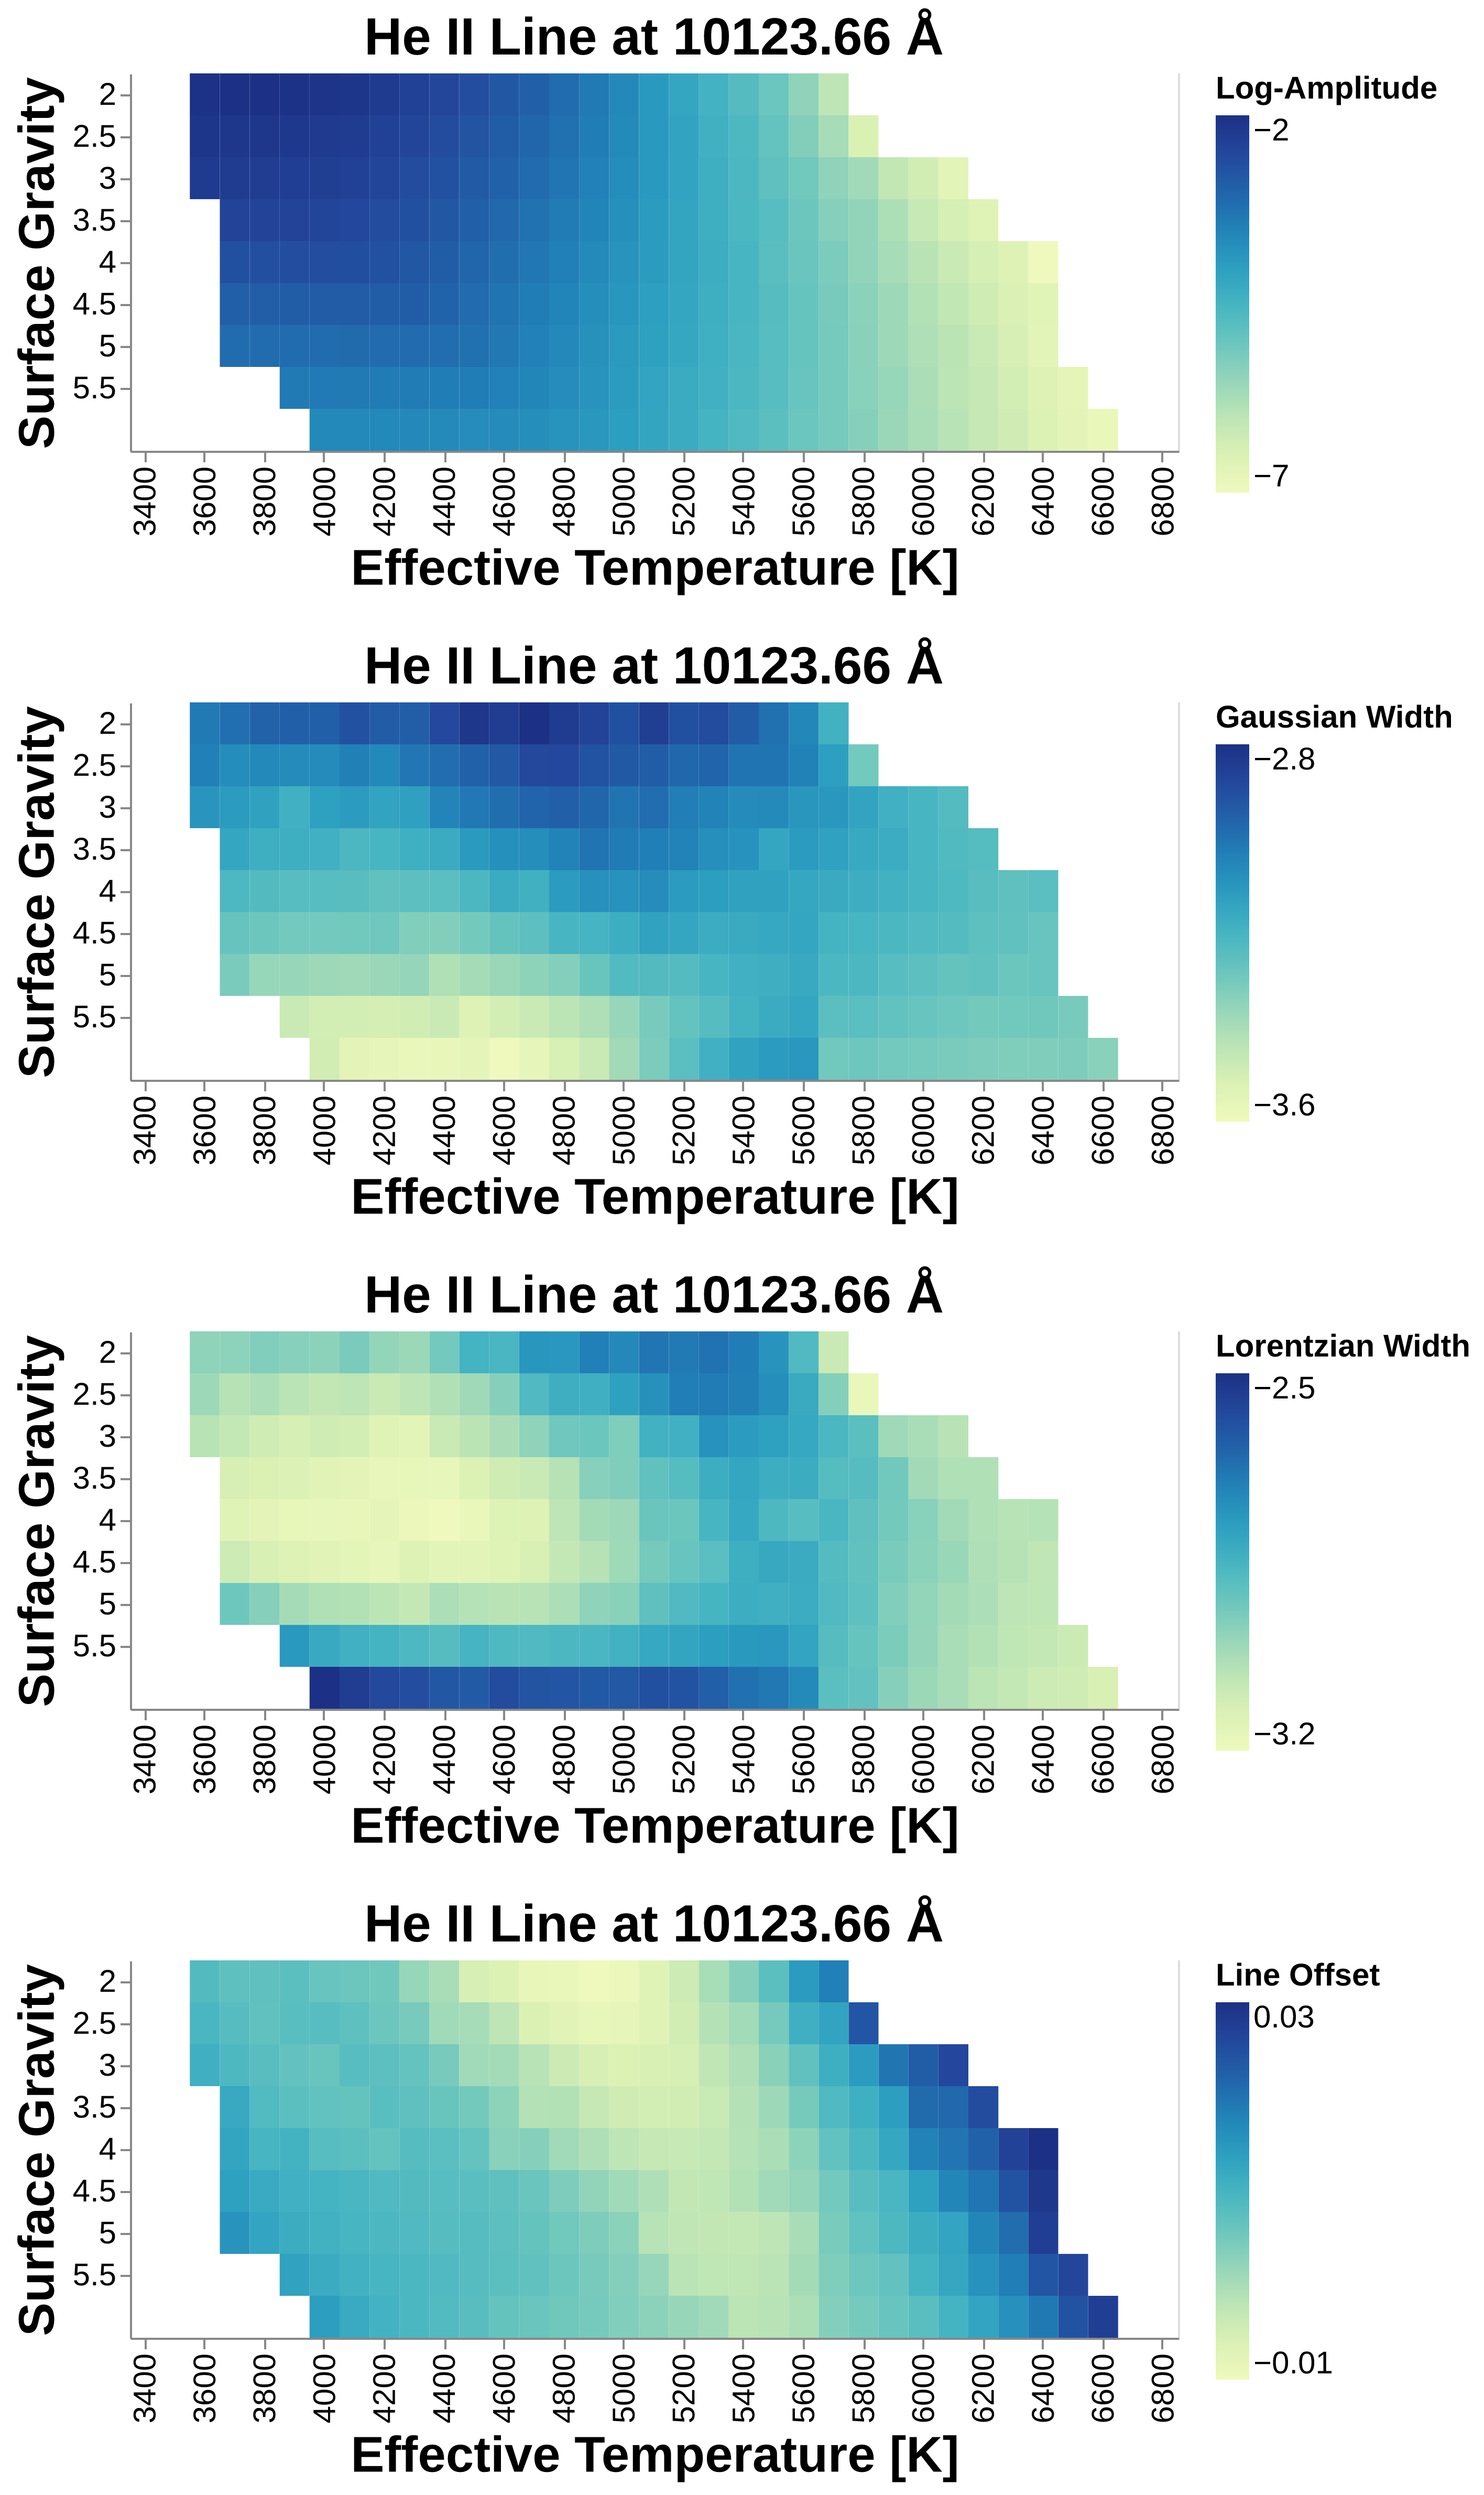
\includegraphics[width=\textwidth]{figure4}
    \caption{Heatmap showing how $\ln(a)$ and $\sigma$ vary over the PHOENIX subset slice at solar metallicity of a He II spectral line.
    We can see that \texttt{blase} detects this line at only a select chunk of grid points in PHOENIX, leading to the large amount of missing data for the line.}
    \label{fig:figure4}
\end{figure*}

\subsection{Continuously Evaluable Manifolds}
For each line, the inputs to the interpolator were the three input parameters $T_{\mathrm{eff}}$, $\log(g)$, and [Fe/H], and the output was a list of four parameters, $\mu'$, $\ln(a)$, $\sigma$, and $\gamma$.
For each line, one of these interpolator objects was created using linear interpolation, and these interpolators were aggregated into a single list, which was then written to disk in the \texttt{.pkl} file storage format.
These interpolators generate multiple manifolds representing the following mapping:
\begin{gather}
    \mqty[T_{\mathrm{eff}} \\ \log(g) \\ \mathrm{[Fe/H]}] \rightarrow \mqty[\mu' \\ \ln(a) \\ \sigma \\ \gamma]
\end{gather}
These interpolators could now be evaluated at any point lying within the domain of the PHOENIX subset, turning a discretely sampled PHOENIX subset into a continuously evaluable function, sometimes called a spectral emulator.
With the given size of the PHOENIX subset, the interpolator list takes up 13.2 GB of disk space.
This evaluation is able to reconstruct an existing PHOENIX spectrum or alternatively interpolate a new spectrum within the domain of the PHOENIX subset, so we call this the PHOENIX generator.
In \autoref{fig:figure5} and \autoref{fig:figure6}, we show the same spectral lines as in \autoref{fig:figure3} and \autoref{fig:figure4}, but now supersampled using the PHOENIX generator evaluated over the same slice.
\begin{figure*}
    \centering
    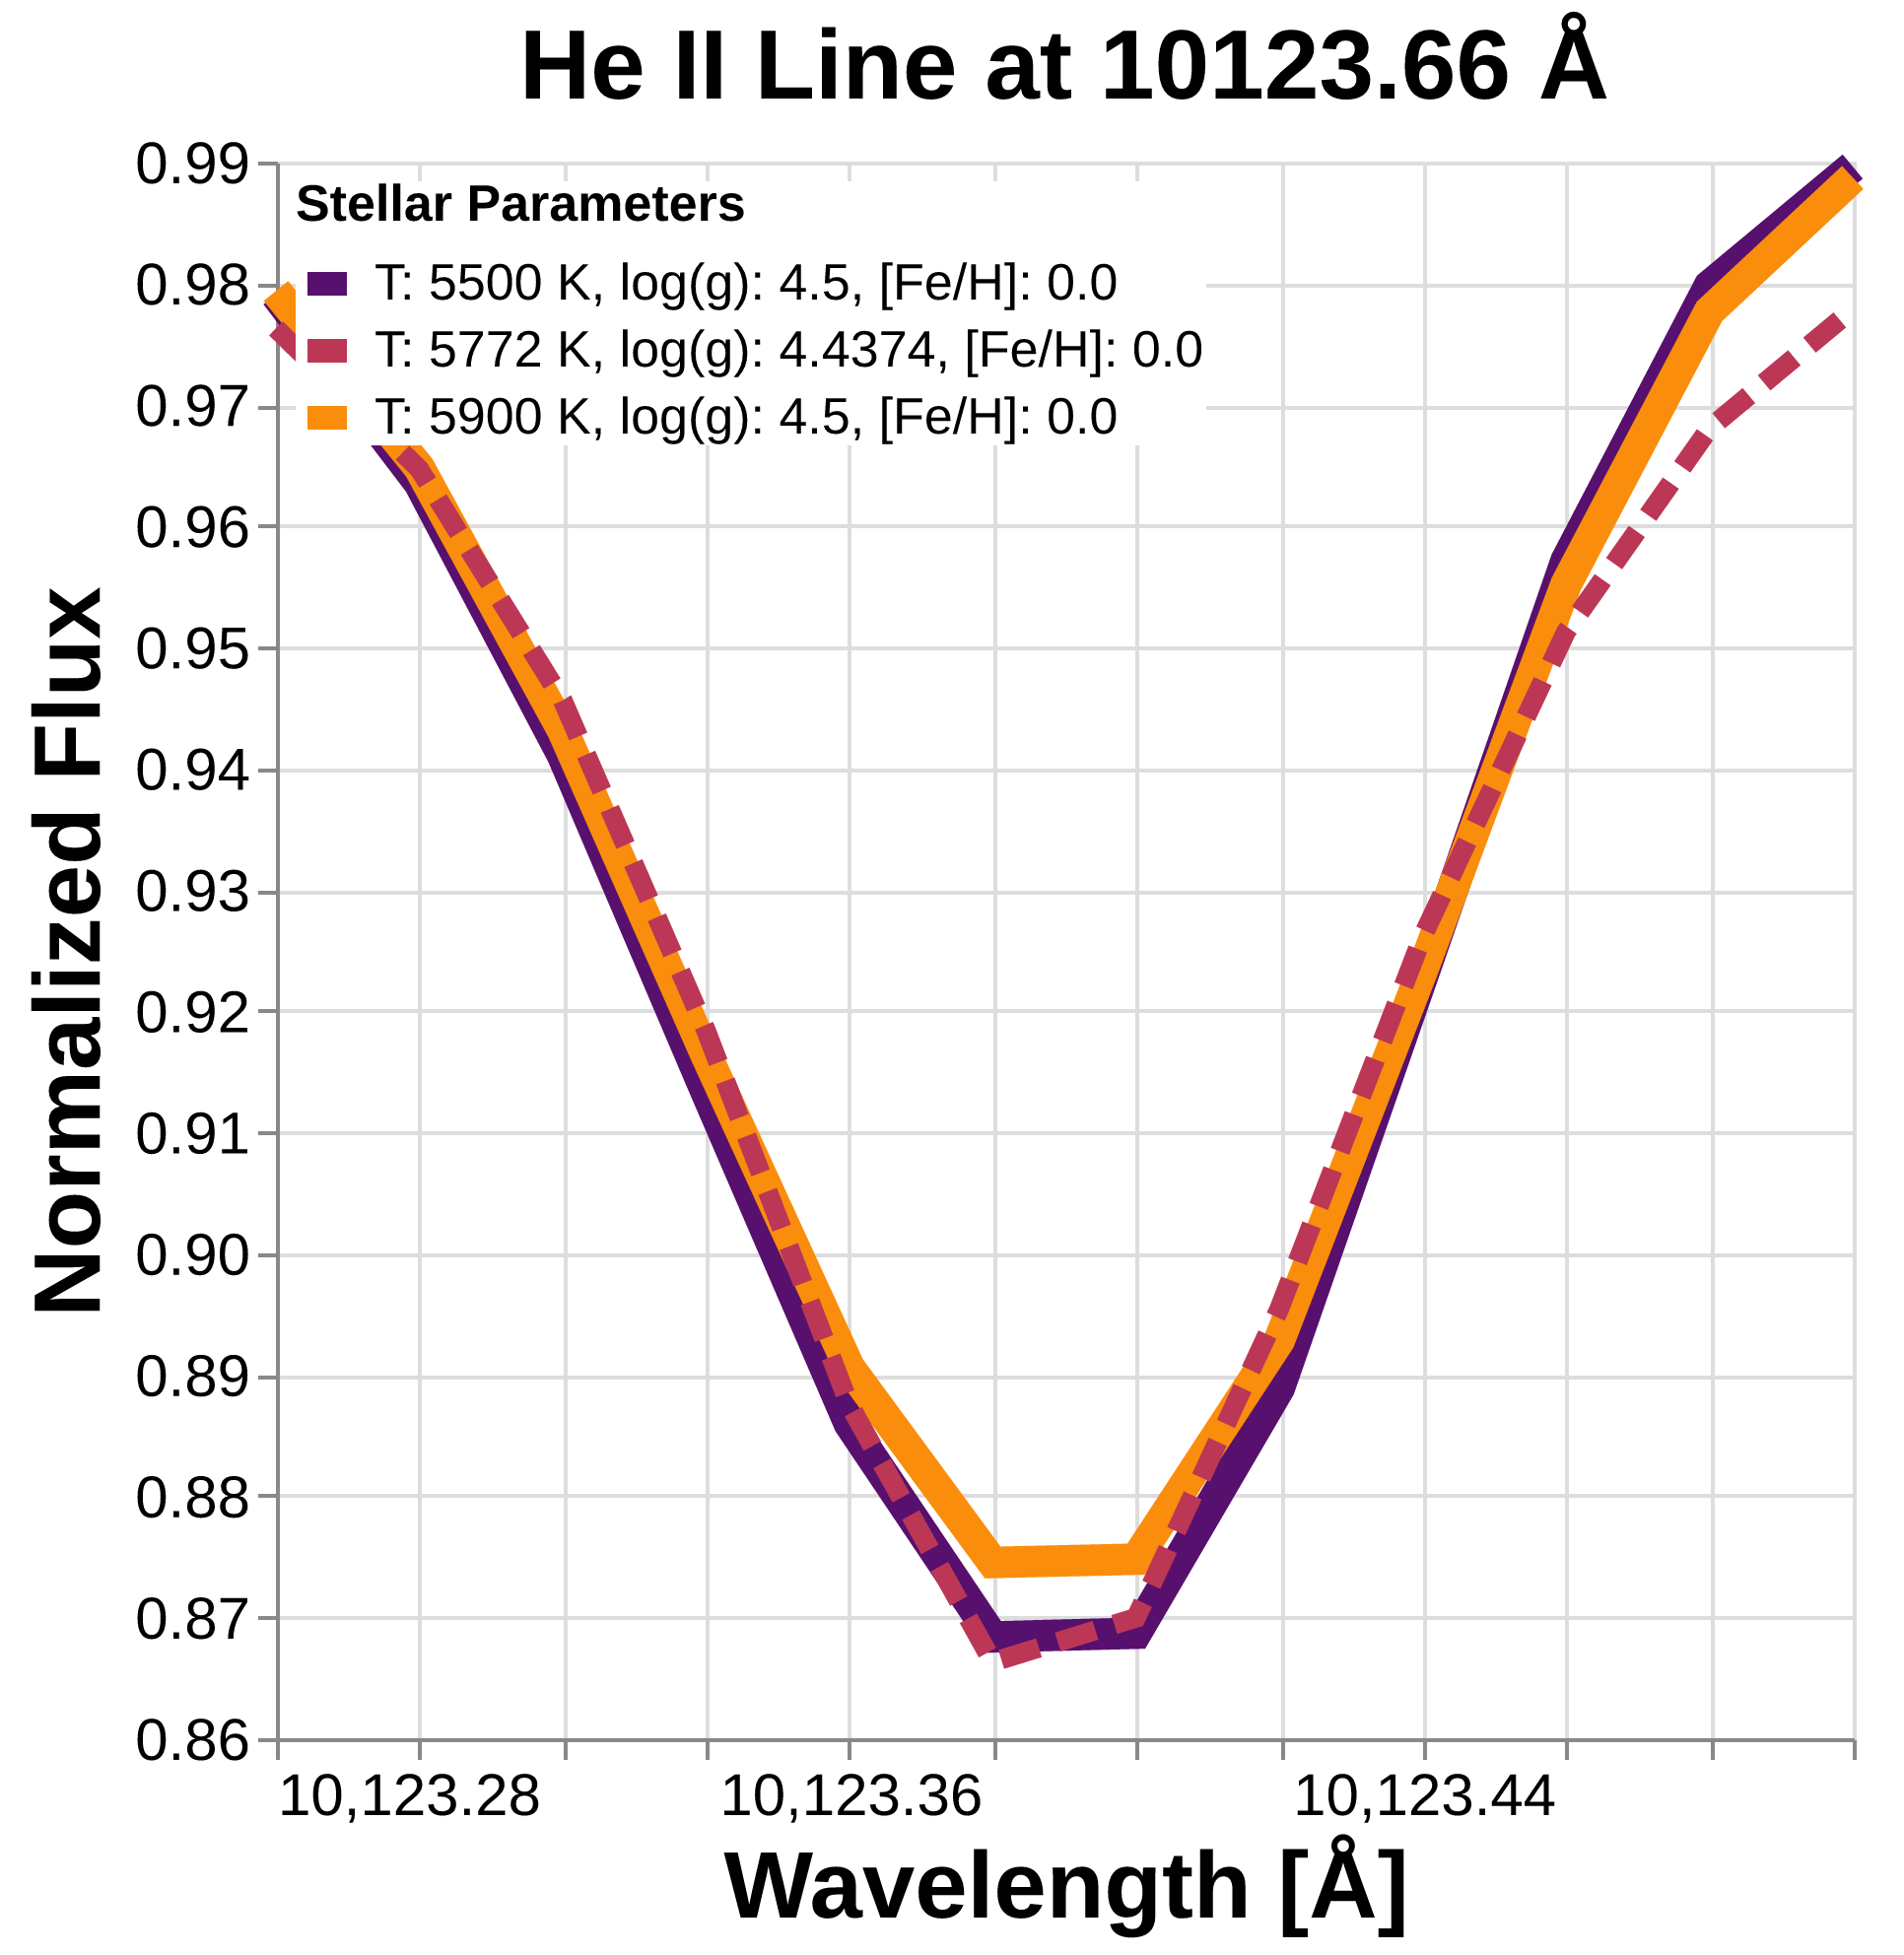
\includegraphics[width=\textwidth]{figure5}
    \caption{Heatmap showing how $\ln(a)$ and $\sigma$ of our \textbf{C I} line vary over the PHOENIX subset slice at solar metallicity, now supersampled with the PHOENIX generator.
    Notice that the missing chunk in the top left still exists and does not display any artifacts, as the artificially populated points are removed after interpolation to retain the model's integrity.
    Also see that the x-axis spacing is now uniform, as the PHOENIX generator was evaluated at constant step.}
    \label{fig:figure5}
\end{figure*}
\begin{figure*}
    \centering
    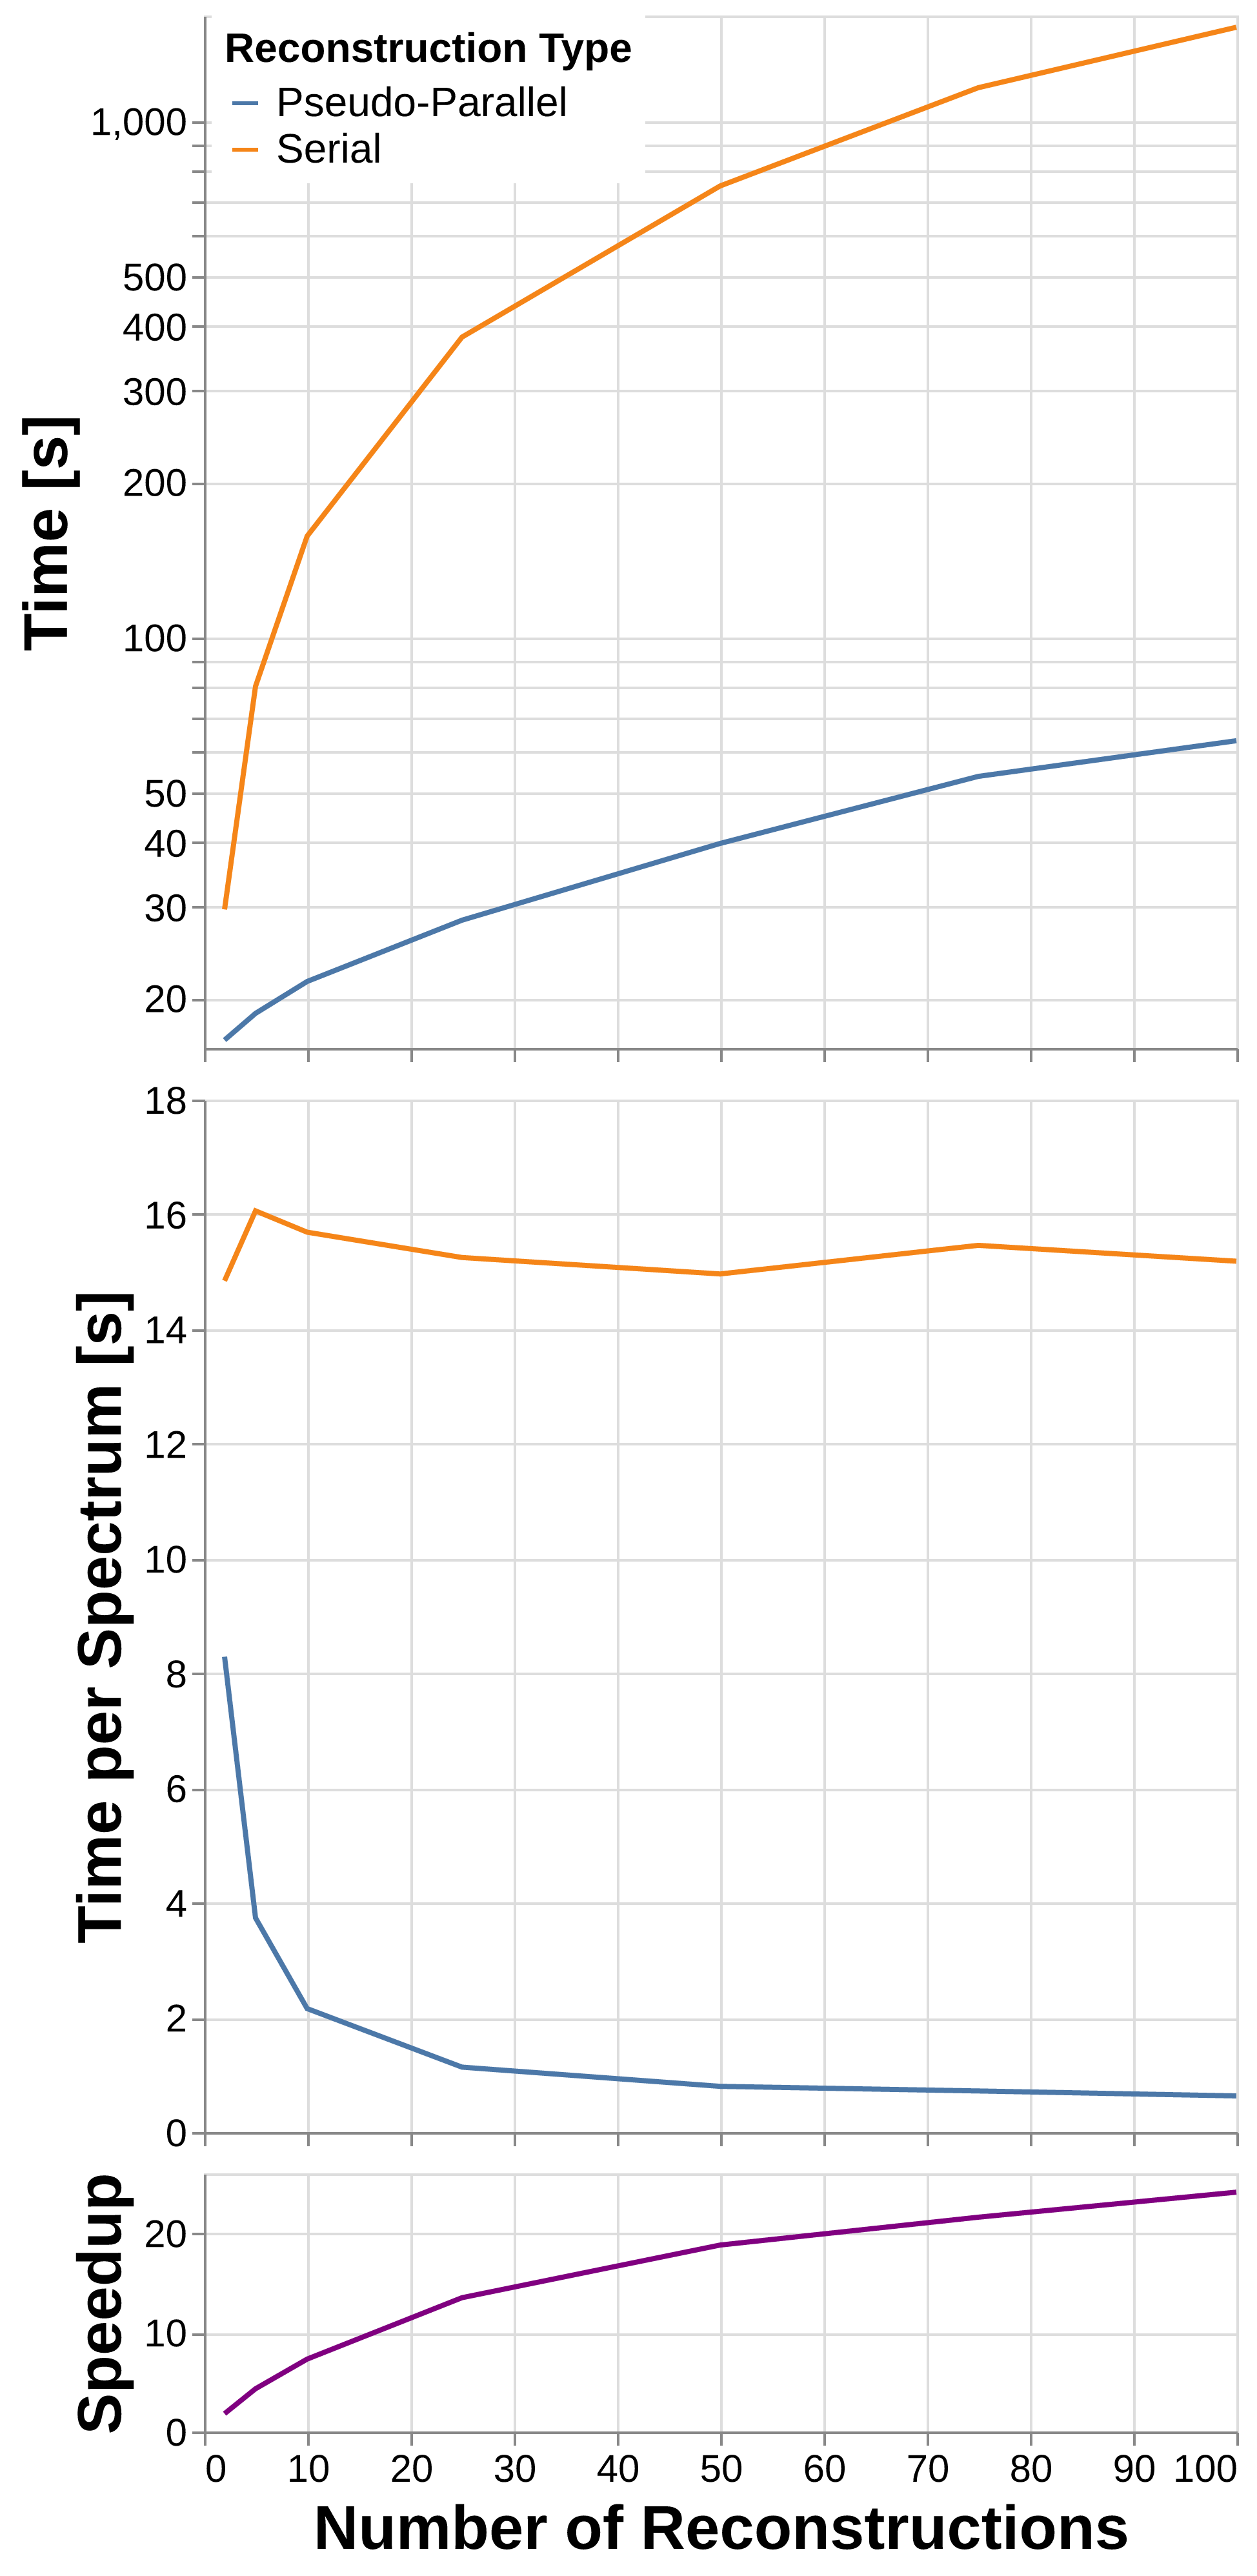
\includegraphics[width=\textwidth]{figure6}
    \caption{Heatmap showing how $\ln(a)$ and $\sigma$ of our He II spectral line vary over the PHOENIX subset slice at solar metallicity, now supersampled with the PHOENIX generator.}
    \label{fig:figure6}
\end{figure*}

The spectral reconstruction process is done by iterating over the PHOENIX generator, evaluating each interpolator at the given coordinates, then reshaping the data into the same format that PyTorch uses for state dictionaries.
During the iteration, if the interpolated log-amplitude of the line is less than -100, the line is excluded from the state dictionary.
We do this to avoid artifacts in the manifolds due to the artifical population of log-amplitudes of -1000 where grid points were missing.

Finally, the state dictionary is fed into \texttt{blase}'s \texttt{SparseLinearEmulator}, which reconstructs the spectrum by constructing a forward model based on the input state dictionary.
Any \texttt{nan} values are set to 1 (which we can do because the spectra are all normalized), and the spectral reconstruction is complete.
\begin{figure*}
    \centering
    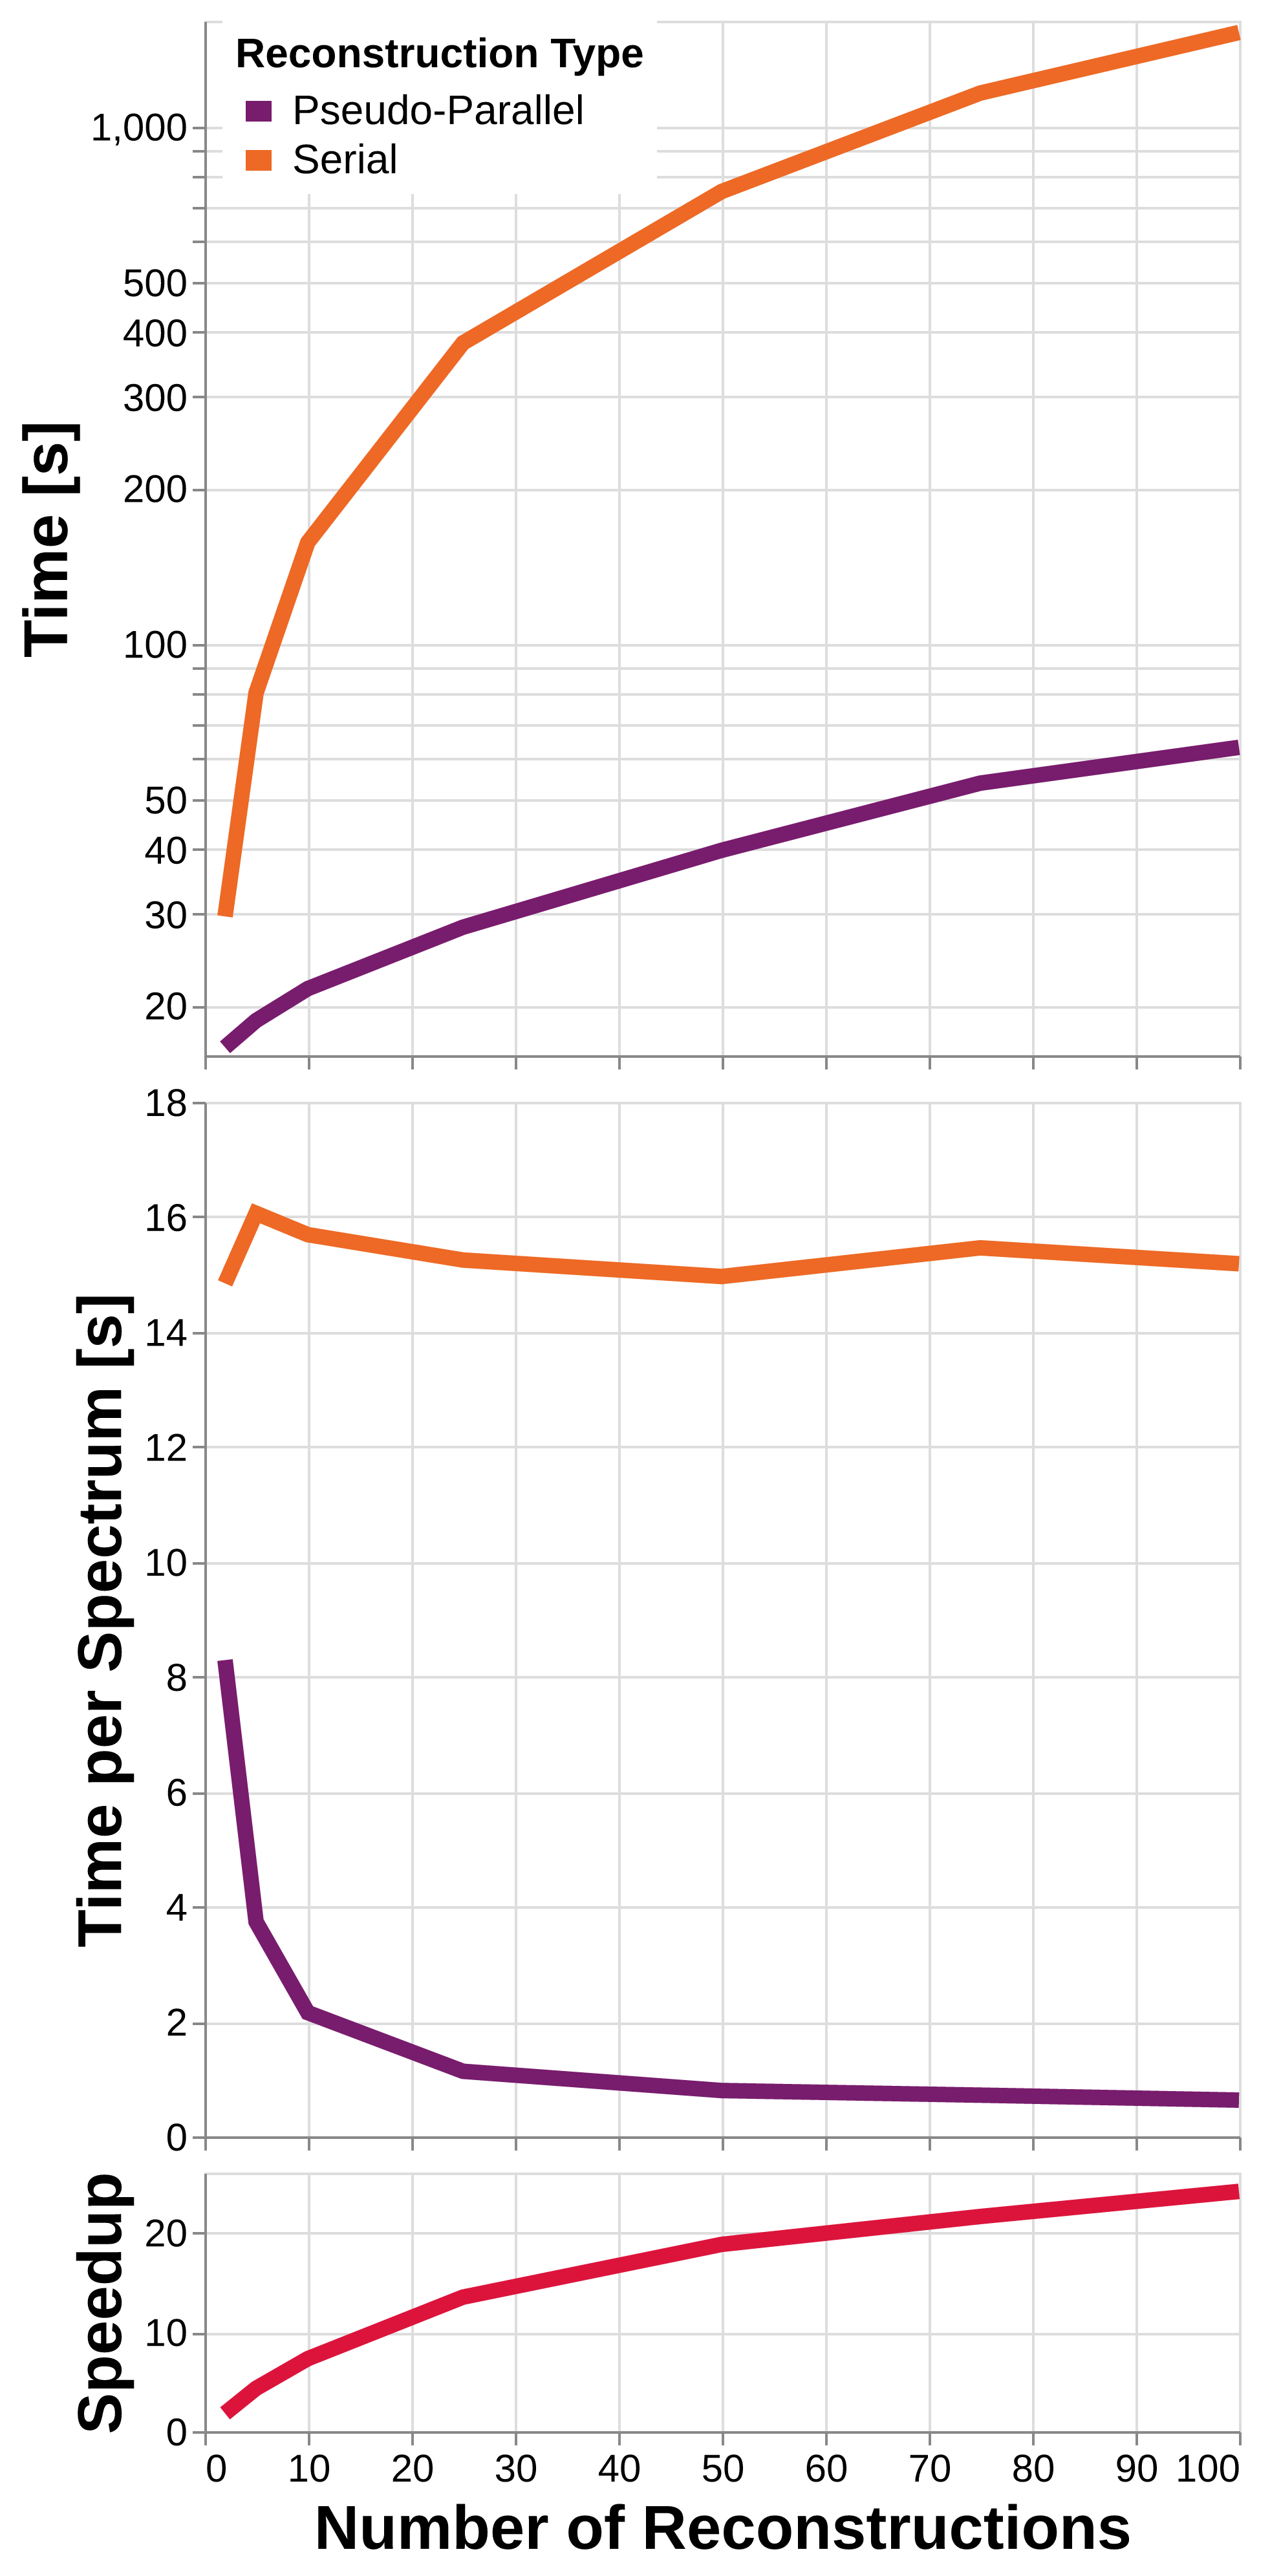
\includegraphics[width=\textwidth]{figure7}
    \caption{Plot of an Fe I spectral line shown at the closest PHOENIX grid points to the Sun's stellar parameters, as well as a solar spectrum reconstructed with the PHOENIX generator.
    We can see the spectral line shape be reconstructed mostly between the two native PHOENIX spectra, being closer to the 5800 K spectrum as the Sun's $T_{\mathrm{eff}}$ used here is 5772 K.}
    \label{fig:figure7}
\end{figure*}
We can observe in \autoref{fig:figure7} that the reconstructed solar spectrum is not simply a pixel interpolation between the nearest grid points.
It is interpolating the spectral line properties using hundreds of thousands of manifolds, each representing a nonlinear parameter in the shape of the spectral line.

\subsection{Spectral Reconstruction Time}
A typical use case for the PHOENIX generator may be to batch reconstruct spectra from an array of input stellar parameters.
Therefore, there is some motivation to reduce the computational cost of this procedure to tractable levels.
We evaluate the computational time needed to use the PHOENIX generator in two distinct ways.
First, for a single input, which would be relevant in serial applications.
Second, for an array of multiple inputs, which would be relevant in parallel applications.
\textbf{\texttt{scipy}'s} \texttt{RegularGridInterpolator} API allows for the passing in of an entire array of input coordinates to be evaluated at once.
However using \texttt{blase} to reconstruct the spectrum from our interpolated state dictionary is always done serially, leading to what is actually more of a pseudo-parallel evaluation, but extremely performant nonetheless.
Performance results are shown in \autoref{fig:figure8}, and we can see that the multi-reconstruction is much faster than a series of single reconstructions.
\textbf{The computer used for this test has the following specifications (note that spectral reconstruction does not currently leverage the GPU):}
\begin{table}[h!]
    \centering
    \begin{tabular}{ll}
        \hline
        CPU & AMD EPYC 7513 (32c/64t, 3.65 GHz boost)\\
        RAM & 256 GB\\
        GPU & Nvidia A100 40GB ($\times$2)\\
        \hline
    \end{tabular}
    \caption{This machine was used for all computations, but not for generating visualizations.}
\end{table}

\begin{figure}[t!]
    \centering
    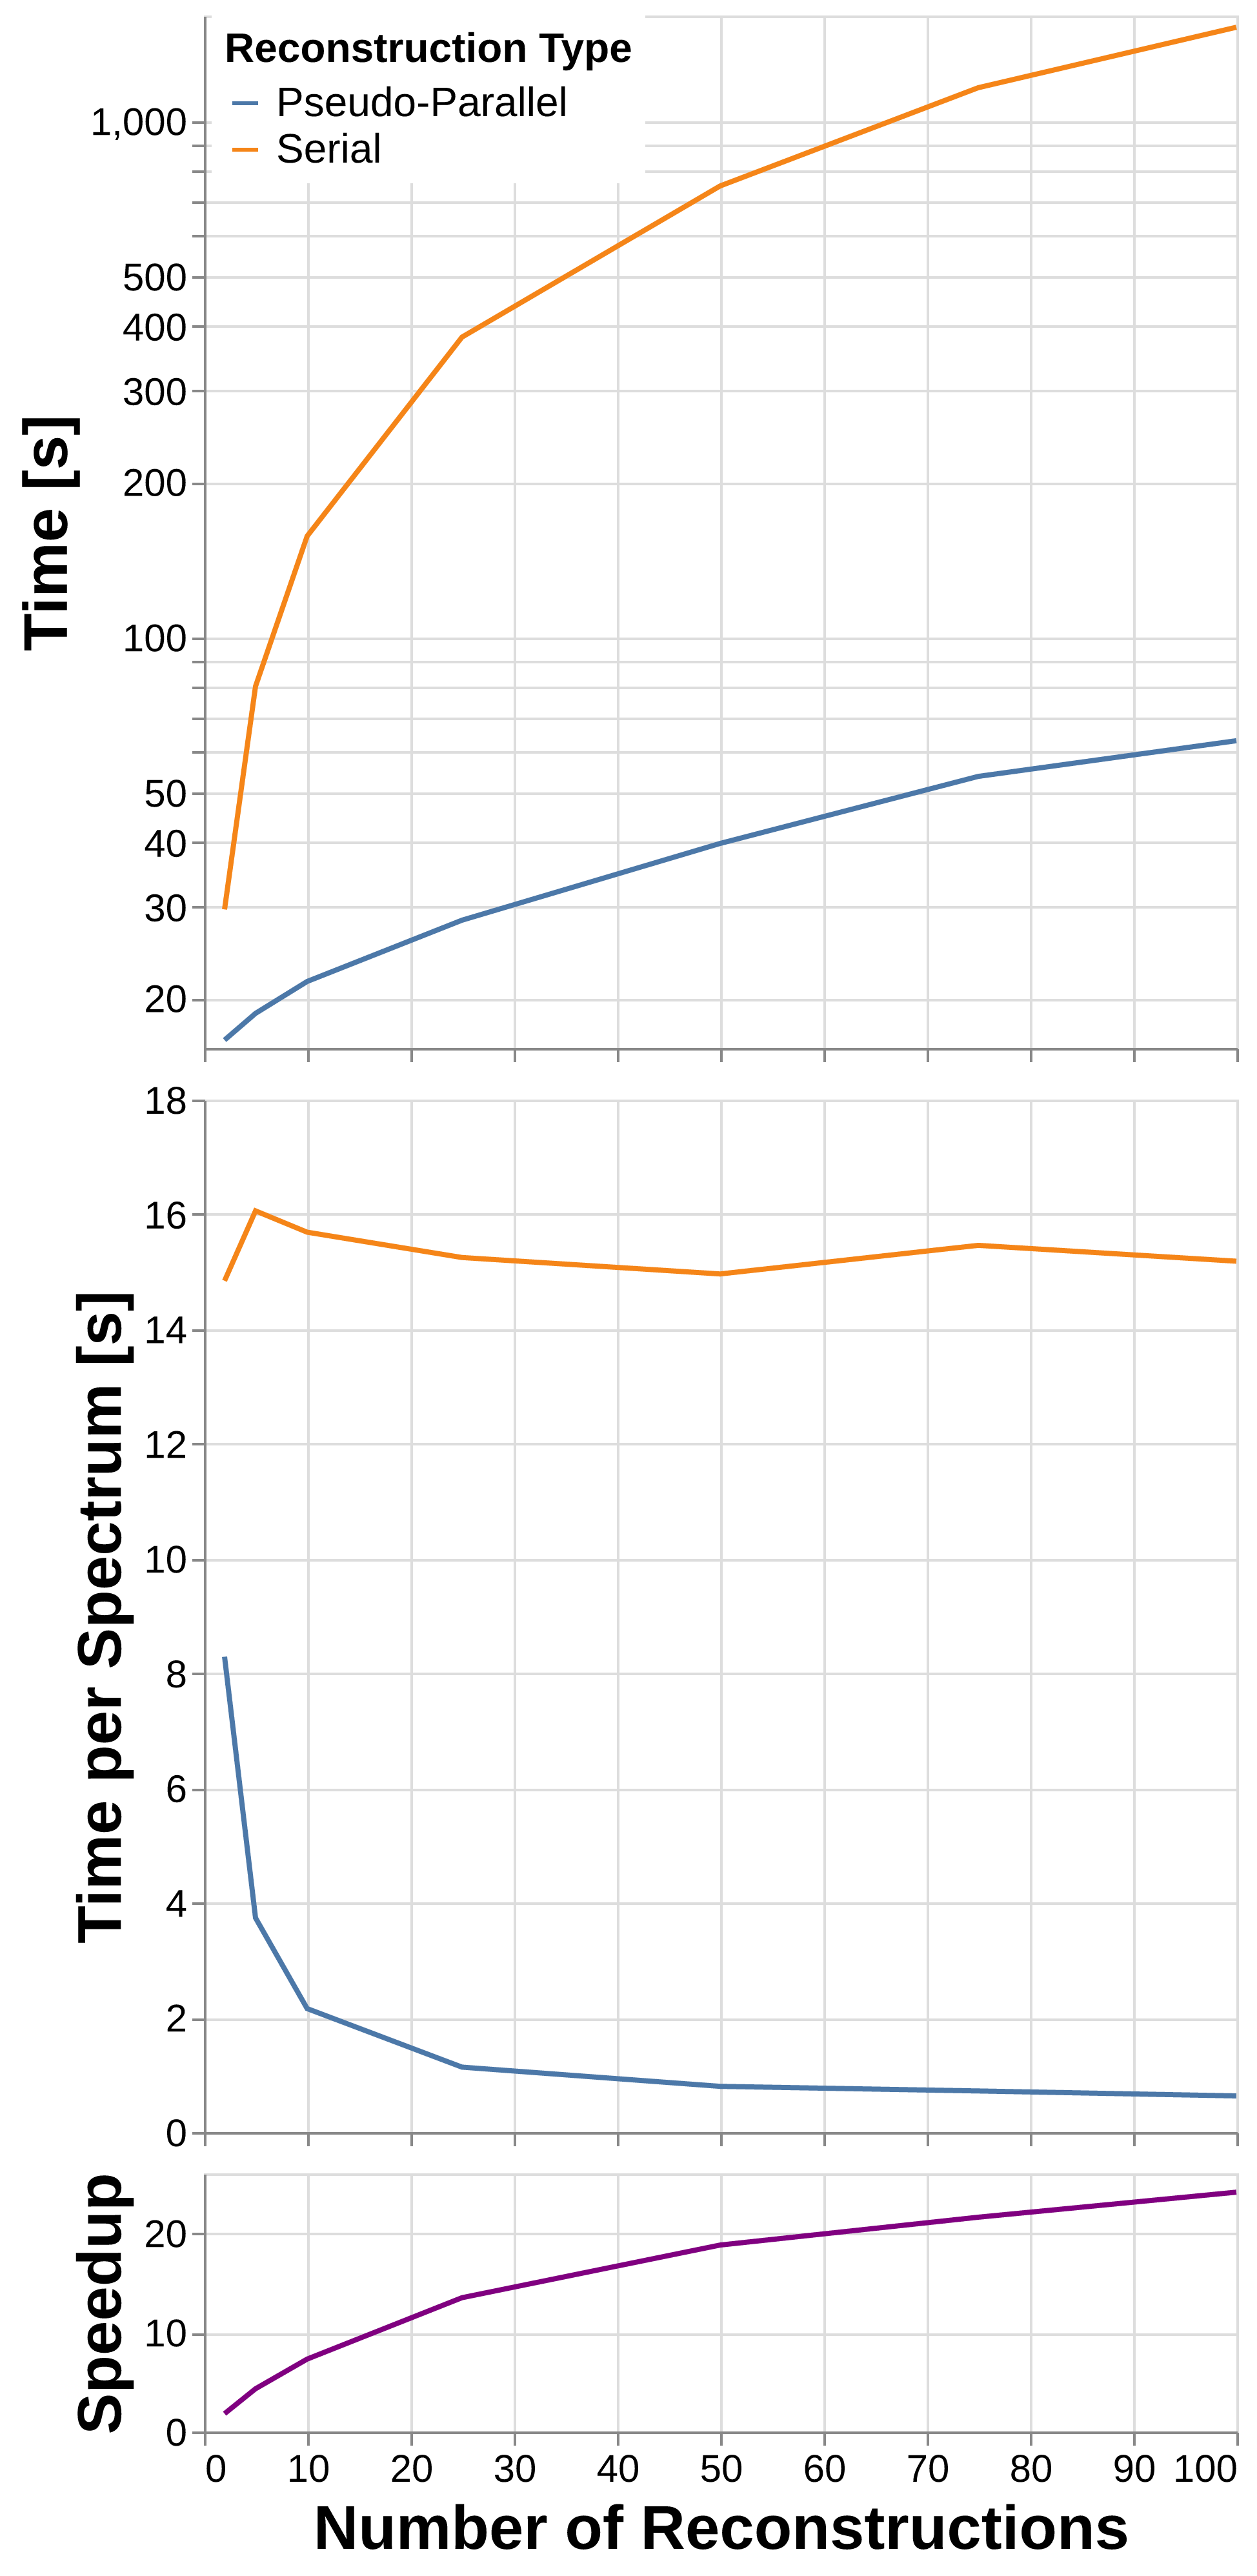
\includegraphics[width=\columnwidth]{figure8}
    \caption{\textbf{Plots} showing the time taken to reconstruct varying numbers of spectra using the PHOENIX generator (lower is better).
    We can see that the time taken per spectr\textbf{um} for the serial implementation hovers around 15 seconds within run-to-run variance, while the pseudo-parallel implementation continually decreases in time taken per spectrum as the number of inputs increases.
    The speedup factor (higher is better) increases as more spectra are generated, which is also a desirable outcome.}
    \label{fig:figure8}
\end{figure}

\section{Bayesian Inference and Testing}
\label{sec:section4}

\subsection{Inference Algorithm}
We elected to use Bayesian optimization as the inference algorithm, specifically the \texttt{gp\_minimize} function from the \texttt{scikit-optimize} library \citep{skopt}.
This algorithm uses a Gaussian Process to model the objective function, which in this case was the RMS (Root-Mean-Square) loss between the interpolated spectrum $\mathsf{M}$ and the true spectrum $\mathsf{D}$, defined as:
\begin{gather}
    \mathcal{L} = \ev{(\mathsf{M} - \mathsf{D})^2}^{1/2}
\end{gather}
The optimizer was configured to first run 100 random evaluations to seed the surrogate model, then run 20 more evaluations now guided by the surrogate model.
This totals to 120 evaluations, a large sample to create a fairly detailed surrogate model, then a moderately precise guided evaluation phase, which was deemed sufficient for this study.
Fine-tuning these numbers is possible, but simply not warranted for a proof-of concept method.
One inference run takes on average just under 7.5 minutes to complete.

\subsection{Bayesian Optimizer Performance}
To test the performance of the inference algorithm, we used the PHOENIX subset itself.
At first glance, this may seem circular, as the PHOENIX generator has memorized the PHOENIX subset, being able to reconstruct a PHOENIX spectrum when evaluated at that grid point.
However, that strategy allows us to use the PHOENIX subset as test data in the context of Bayesian optimization.
The \texttt{gp\_minimize} surrogate model is seeded by random continuously sampled generator evaluations within the search space, \textit{not} grid points of the PHOENIX subset, meaning the surrogate model has no memorization to speak of.
If the optimizer had been a grid-based strategy, this would not have been possible, because then the surrogate model would be affected by memorization.

We know that in typical observational settings, a coarse estimate for $T_{\mathrm{eff}}$ tends to be fairly well-constrained from ancillary data \textbf{such as photometric color index}.
So when testing the inference algorithm, we limited its search space to only include $T_{\mathrm{eff}}$ which lay within 500 K of the true value on either side.
$\log(g)$ and [Fe/H] were allowed to vary freely.
The test sample consisted of 9 unique $T_{\mathrm{eff}}$ values, 3 unique $\log(g)$ values, and 2 unique [Fe/H] values, totaling 54 unique spectra in the test set.
$T_{\mathrm{eff}}$ ranged from 3000 K to 11000 K in increments of 1000 K, $\log(g)$ ranged from 2 to 6 in increments of 2, and [Fe/H] ranged from -0.5 to 0 in increments of 0.5.

The results of the inference algorithm are as follows: $T_{\mathrm{eff}}$ differed from the true result by an average of 185 K or 2.6\%.
$\log(g)$ differed by an average of 0.19 or 6.8\%. [Fe/H] differed by an average of 0.12 dex, which is 24\% of our search range.
From this, we can see that $T_{\mathrm{eff}}$ was the most accurately inferred parameter, followed by $\log(g)$, and then [Fe/H].

\section{Discussion}
\subsection{Scientific Applications}
This study's paradigm of spectral inference can enable scientists to adopt self-consistent model grids and analyze their spectral line behavior in an interpretable fashion, which has been fairly uncommon practice thus far.
Notably, this system tracks the shifting of spectral lines as a function of stellar parameters, which traditionally has been uncommon for algorithms to assess systematically.
We balance rigidity and flexibility where we want them while maintaining interpretability.

To summarize, we bring to scientists the ability to understand exactly what spectral properties we consider mathematically and how we expect those properties to behave on an incredibly detailed level (the 4 line parameters of all spectral lines and their corresponding interpolating manifolds), and introduce the concept of postulating one precomputed model grid as the ground truth to base all further analysis on, converting the grid into a generator that can then interface with our inference algorithm.

\subsection{Technical Considerations}
To reiterate, the manifold fitting steps are not end-to-end autodifferentiable.
As seen in \autoref{fig:figure1}, these steps rely on \texttt{scipy}, which is not equipped with autodiff.
Without autodifferentiability, the ability to ``machine learn'' is significantly reduced compared to a hypothetical monolithic JAX or PyTorch system.
We see three reasons for for developing a non-autodifferentiable system.
First, the familiar \texttt{scipy}-based system will serve as an easy entry point for most practitioners who are unfamiliar with autodiff, and may still benefit from and modify the code without expert ML knowledge.
Second, this non-autodiff version serves as a\textbf{n initial} benchmark against which an inevitable autodifferentiable version may be compared.
Finally, the inventory of familiar interpolation algorithms have not yet been ported to PyTorch or JAX, since machine learning or Gaussian Process fitting schemes are generally preferred within the ML community.

The interpolation scheme presented here represents a proof of concept, showing that leveraging the mapping between synthetic spectral lines and their inputs can yield a semi-empirical basis for data-model comparisons.
There are numerous design considerations that could be improved upon with future work.
These include but are not limited to the following:
\begin{enumerate}[label=-]
    \item \textit{Limited PHOENIX Subset}: The PHOENIX subset used in this study did not include the full PHOENIX grid, which expands the [Fe/H] range to [-4.0, 1.0] dex and the $\log(g)$ range to [0, 6], and also includes the alpha element abundance parameter, which we elected to fix at 0 for this study.
    In addition to the actual stellar parameters, we also took a subset of the PHOENIX wavelength range, with the full [500, 55000] \AA \ wavelength range also being left to future work.
    Users would be able to fit a greater variety of stellar spectra in many different wavelength regimes.
    \item \textit{Strict Wavelength Range}: Currently, the generator only supports inference on spectra whose wavelength limits are either equal to it, or encompass that of the generator and have been truncated to match.
    However, when the spectrum in question has a smaller wavelength range than the generator, currently there is no functionality to truncate the generator.
    This would require externally indexing the generator's individual interpolators by line center position and selectively evaluating those to eliminate wasteful computation.
    This takes burden off the users to truncate their data to the PHOENIX generators, making use simpler.
    \item \textit{Single Model Grid}: The PHOENIX grid is not the only model grid of synthetic spectra available, and it does not apply to all types of stars.
    Future work would extend the reach of this study's algorithm to encompass other model grids such as the Sonora series of substellar models \textbf{\citep{bobcat, cholla, diamondback, elfowl}}, ATLAS \citep{atlas}, and coolTLUSTY \citep{coolTLUSTY}, reaching practitioners studying various types of stars and spectra.
    \textbf{Future} \texttt{blase} \textbf{versions will} be able to have an option for the user to input which model grid they would like to base the inference on, and to get even more advanced, perhaps even have the ability to intelligently determine which model grid to use automatically.
    \item \textit{Memorization vs.\ Generalization}: The current design of the algorithm constructs manifolds using interpolation.
    This means that performance is good at points close to PHOENIX subset grid points, but is highly dependent on the type of interpolation used.
    As interpolators require memorization of the data, advanced interpolation becomes extremely expensive in terms of disk utilization.
    Future work would involve constructing manifolds using \textbf{more generalizable ML} methods \textbf{such as lasso or ridge regression}, which would allow for much better generalization, high speed, and lower disk utilization at the expense of some accuracy.
    \item \textit{Extrinsic Absence}: The current design of our algorithm does not account for extrinsic parameters that modify the appearance of spectra such as rotational broadening and Doppler shifting.
    Future work would need to develop ways to tune these extrinsic parameters alongside stellar parameters, enabling users to optimize these frequently-observed extrinsic parameters on top of the base stellar parameters.
    \item \textit{Framework Overhead}: As this algorithm is currently more proof of concept than practical, it uses convenience functions from various libraries, which naturally introduces some level of overhead and leaves performance on the table.
    Future work would involve writing custom functions expressly designed for \texttt{blase}, most likely a complete rewrite of the library from the ground up.
    This has the potential to greatly increase the speed of this algorithm, depending on how much overhead is avoided with a bespoke implementation.
    \item \textit{Pseudo-Interpretability}: Our algorithm boasts interpretability by considering spectral lines as the objects of interest as opposed to the rather uninterpretable flux values of other approaches.
    However, this is only a step in the direction of interpretability.
    True interpretability would decompose a spectrum not into a set of spectral lines, but into a set of species component spectra, which requires a much more advanced understanding of different species and their behavior, as well as direct access to a radiative transfer code as opposed to an off-the-shelf model grid.
    This approach would also extend the inference from just stellar parameters defined by a grid to any set of parameters accounted for in the radiative transfer model, down to specific species abundances.
    So while we were able to identify the spectral lines used in our figures, it is not necessarily valuable to try to identify all 128,723 lines that we identify as unique with our algorithm.
    \texttt{blase} is \textit{agnostic} to the identity of the line that it is optimizing.
    We study these lines as \texttt{blase} sees them (i.e. their four shape parameters), because for the purposes of this study, that is the only information that is useful.
    Having more interpretability would let scientists actually study certain species and their spectral lines.
    \item \textit{The Continuum Black Box}: Continuum normalization is a process that is not yet completely understood, and is currently done as a preprocessing step with a fairly simple algorithm.
    Future work would dive deeper into the science of continu\textbf{a} and develop more advanced methods that can discern continu\textbf{a} with greater accuracy and less modeling restrictions.
    This would increase accuracy for end users.
    \item \textit{One Voigt Fits All}: The current assumption of \texttt{blase} is that every spectral line is a Voigt profile.
    This assumption is largely true, but there are situations where that is simply not enough.
    Future studies need to account for more advanced spectral line profiles and procedures to deal with phenomena such as ro-vibrational bands.
    This would increase accuracy for end users.
\end{enumerate}

\section{Conclusion}
In this study, we have presented a proof-of-concept algorithm that interpolates a subset of the PHOENIX spectral model grid and then uses GP minimization \textbf{to infer stellar paremeters}.
We create state dictionaries for all spectra in the PHOENIX subset, lossily distilling the spectra with a data compression factor of around 20. 
The\textbf{y are available on} Zenodo at \url{https://zenodo.org/records/11246174} \citep{zenodo}.
We create the PHOENIX generator and implement a performant spectral reconstruction algorithm, enabling anyone to create reconstructions of PHOENIX spectra with continuously valued stellar parameters.
We introduce and test our inference algorithm, with average absolute deviations from true values of 185 K in $T_\mathrm{eff}$, 0.19 in $\log(g)$, and 0.12 dex in [Fe/H].
In its current state, our algorithm operates on spectra within the PHOENIX subset parameter ranges in \autoref{tab:table1}, requiring that the spectra not contain noticeable Doppler shifting, rotational broadening, or other confounding factors.
The methods discussed here represent a step down a road not traveled in spectral inference, and have the potential to become more advanced in the future by fully utilizing the strengths of physics-informed machine learning.

\vspace{0.5cm}
This material is based on work supported by the National Aeronautics and Space Administration under grant No. 80NSSC21K0650 for the NNH20ZDA001N-ADAP:D.2 program. C.V.M. acknowledges support from the Alfred P. Sloan Foundation under grant number FG-2021-16592 and support from the National Science Foundation under grant number 1910969.
\vspace{0.5cm}

\software{
    \texttt{altair} \citep{altair1, altair2},
    \texttt{astropy} \citep{astropy1, astropy2, astropy3},
    blas\'e/\texttt{blase} \citep{blase},
    CUDA \citep{cuda},
    \texttt{gollum} \citep{gollum},
    \texttt{matplotlib} \citep{mpl},
    \texttt{numpy} \citep{numpy},
    \texttt{pandas} \citep{pandas1, pandas2},
    Python \citep{python},
    PyTorch/\texttt{torch} \citep{pytorch},
    scikit-optimize/\texttt{skopt} \citep{skopt},
    \texttt{scipy} \citep{scipy},
    \texttt{tqdm} \citep{tqdm},
    \texttt{vegafusion} \citep{vegafusion},
}

\bibliography{paper}

\end{document}
